\documentclass[11pt]{article}

\newcommand{\yourname}{Kevin Zhang}

\def\comments{0}

%format and packages

%\usepackage{algorithm, algorithmic}
\usepackage{tikz}
\usepackage{algpseudocode}
\usepackage{amsmath, amssymb, amsthm}
\usepackage{tcolorbox}
\usepackage{enumerate}
\usepackage{enumitem}
\usepackage{framed}
\usepackage{verbatim}
\usepackage[margin=1.0in]{geometry}
\usepackage{microtype}
\usepackage{kpfonts}
\usepackage{palatino}
	\DeclareMathAlphabet{\mathtt}{OT1}{cmtt}{m}{n}
	\SetMathAlphabet{\mathtt}{bold}{OT1}{cmtt}{bx}{n}
	\DeclareMathAlphabet{\mathsf}{OT1}{cmss}{m}{n}
	\SetMathAlphabet{\mathsf}{bold}{OT1}{cmss}{bx}{n}
	\renewcommand*\ttdefault{cmtt}
	\renewcommand*\sfdefault{cmss}
	\renewcommand{\baselinestretch}{1.06}

\usepackage[boxruled,vlined,nofillcomment]{algorithm2e}
	\SetKwProg{Fn}{Function}{\string:}{}
	\SetKwFor{While}{While}{}{}
	\SetKwFor{For}{For}{}{}
	\SetKwIF{If}{ElseIf}{Else}{If}{:}{ElseIf}{Else}{:}
	\SetKw{Return}{Return}
	

%enclosure macros
\newcommand{\paren}[1]{\ensuremath{\left( {#1} \right)}}
\newcommand{\bracket}[1]{\ensuremath{\left\{ {#1} \right\}}}
\renewcommand{\sb}[1]{\ensuremath{\left[ {#1} \right\]}}
\newcommand{\ab}[1]{\ensuremath{\left\langle {#1} \right\rangle}}

%probability macros
\newcommand{\ex}[2]{{\ifx&#1& \mathbb{E} \else \underset{#1}{\mathbb{E}} \fi \left[#2\right]}}
\newcommand{\pr}[2]{{\ifx&#1& \mathbb{P} \else \underset{#1}{\mathbb{P}} \fi \left[#2\right]}}
\newcommand{\var}[2]{{\ifx&#1& \mathrm{Var} \else \underset{#1}{\mathrm{Var}} \fi \left[#2\right]}}

%useful CS macros
\newcommand{\poly}{\mathrm{poly}}
\newcommand{\polylog}{\mathrm{polylog}}
\newcommand{\zo}{\{0,1\}}
\newcommand{\pmo}{\{\pm1\}}
\newcommand{\getsr}{\gets_{\mbox{\tiny R}}}
\newcommand{\card}[1]{\left| #1 \right|}
\newcommand{\set}[1]{\left\{#1\right\}}
\newcommand{\negl}{\mathrm{negl}}
\newcommand{\eps}{\varepsilon}
\DeclareMathOperator*{\argmin}{arg\,min}
\DeclareMathOperator*{\argmax}{arg\,max}
\newcommand{\eqand}{\qquad \textrm{and} \qquad}
\newcommand{\ind}[1]{\mathbb{I}\{#1\}}
\newcommand{\sslash}{\ensuremath{\mathbin{/\mkern-3mu/}}}

%mathbb
\newcommand{\N}{\mathbb{N}}
\newcommand{\R}{\mathbb{R}}
\newcommand{\Z}{\mathbb{Z}}
%mathcal
\newcommand{\cA}{\mathcal{A}}
\newcommand{\cB}{\mathcal{B}}
\newcommand{\cC}{\mathcal{C}}
\newcommand{\cD}{\mathcal{D}}
\newcommand{\cE}{\mathcal{E}}
\newcommand{\cF}{\mathcal{F}}
\newcommand{\cL}{\mathcal{L}}
\newcommand{\cM}{\mathcal{M}}
\newcommand{\cO}{\mathcal{O}}
\newcommand{\cP}{\mathcal{P}}
\newcommand{\cQ}{\mathcal{Q}}
\newcommand{\cR}{\mathcal{R}}
\newcommand{\cS}{\mathcal{S}}
\newcommand{\cU}{\mathcal{U}}
\newcommand{\cV}{\mathcal{V}}
\newcommand{\cW}{\mathcal{W}}
\newcommand{\cX}{\mathcal{X}}
\newcommand{\cY}{\mathcal{Y}}
\newcommand{\cZ}{\mathcal{Z}}

%theorem macros
\newtheorem{thm}{Theorem}
\newtheorem{lem}[thm]{Lemma}
\newtheorem{fact}[thm]{Fact}
\newtheorem{clm}[thm]{Claim}
\newtheorem{rem}[thm]{Remark}
\newtheorem{coro}[thm]{Corollary}
\newtheorem{prop}[thm]{Proposition}
\newtheorem{conj}[thm]{Conjecture}

\theoremstyle{definition}
\newtheorem{defn}[thm]{Definition}
\newtheoremstyle{case}{}{}{}{}{}{:}{ }{}
\theoremstyle{case}
\newtheorem{case}{Case}

\theoremstyle{theorem}
\newtheorem{prob}{Problem}
\newtheorem{sol}{Solution}

\tikzset{every picture/.style={line width=0.75pt}} %set default line width to 0.75pt        

\begin{document}
{\large
\noindent Name: \yourname}

\vspace{15pt}

\begin{prob}\end{prob}

Problem will be submitted through tint homework submission. Placeholder for correct problem numbering.

\begin{prob}\end{prob}

\begin{enumerate}[label=(\alph*)]

\item
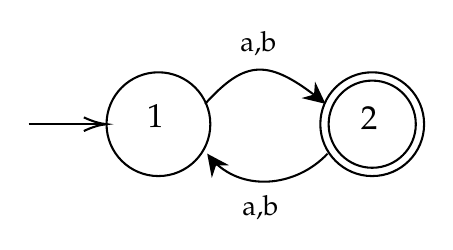
\begin{tikzpicture}[x=0.75pt,y=0.75pt,yscale=-1,xscale=1]
%uncomment if require: \path (0,130); %set diagram left start at 0, and has height of 130

%Shape: Circle [id:dp9201741477235257] 
\draw   (57,63) .. controls (57,49.19) and (68.19,38) .. (82,38) .. controls (95.81,38) and (107,49.19) .. (107,63) .. controls (107,76.81) and (95.81,88) .. (82,88) .. controls (68.19,88) and (57,76.81) .. (57,63) -- cycle ;
%Shape: Circle [id:dp9942563467001306] 
\draw   (164,63) .. controls (164,51.4) and (173.4,42) .. (185,42) .. controls (196.6,42) and (206,51.4) .. (206,63) .. controls (206,74.6) and (196.6,84) .. (185,84) .. controls (173.4,84) and (164,74.6) .. (164,63) -- cycle ;
%Shape: Circle [id:dp694035962297272] 
\draw   (160,63) .. controls (160,49.19) and (171.19,38) .. (185,38) .. controls (198.81,38) and (210,49.19) .. (210,63) .. controls (210,76.81) and (198.81,88) .. (185,88) .. controls (171.19,88) and (160,76.81) .. (160,63) -- cycle ;
%Curve Lines [id:da7011253414000169] 
\draw    (104.5,53.2) .. controls (124,31.75) and (134.94,31.21) .. (160.5,51.59) ;
\draw [shift={(162.5,53.2)}, rotate = 219.17000000000002] [fill={rgb, 255:red, 0; green, 0; blue, 0 }  ][line width=0.08]  [draw opacity=0] (10.72,-5.15) -- (0,0) -- (10.72,5.15) -- (7.12,0) -- cycle    ;
%Straight Lines [id:da18565194669449947] 
\draw    (19.5,63) -- (55,63) ;
\draw [shift={(57,63)}, rotate = 180] [color={rgb, 255:red, 0; green, 0; blue, 0 }  ][line width=0.75]    (10.93,-3.29) .. controls (6.95,-1.4) and (3.31,-0.3) .. (0,0) .. controls (3.31,0.3) and (6.95,1.4) .. (10.93,3.29)   ;
%Curve Lines [id:da8222805136433349] 
\draw    (163.5,77.2) .. controls (148.14,93.52) and (121.72,96.02) .. (107.25,79.38) ;
\draw [shift={(105.5,77.2)}, rotate = 413.62] [fill={rgb, 255:red, 0; green, 0; blue, 0 }  ][line width=0.08]  [draw opacity=0] (10.72,-5.15) -- (0,0) -- (10.72,5.15) -- (7.12,0) -- cycle    ;

% Text Node
\draw (75,52) node [anchor=north west][inner sep=0.75pt]  [font=\large] [align=left] {1};
% Text Node
\draw (178,53) node [anchor=north west][inner sep=0.75pt]  [font=\large] [align=left] {2};
% Text Node
\draw (120,17) node [anchor=north west][inner sep=0.75pt]   [align=left] {a,b};
% Text Node
\draw (121,96) node [anchor=north west][inner sep=0.75pt]   [align=left] {a,b};
\end{tikzpicture}

where 1 is the state of even length, and 2 is the state of odd length.

\item

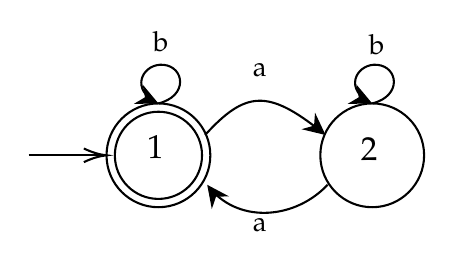
\begin{tikzpicture}[x=0.75pt,y=0.75pt,yscale=-1,xscale=1]
%uncomment if require: \path (0,112); %set diagram left start at 0, and has height of 112

%Shape: Circle [id:dp3548753250718797] 
\draw   (57,62) .. controls (57,48.19) and (68.19,37) .. (82,37) .. controls (95.81,37) and (107,48.19) .. (107,62) .. controls (107,75.81) and (95.81,87) .. (82,87) .. controls (68.19,87) and (57,75.81) .. (57,62) -- cycle ;
%Shape: Circle [id:dp802968937091256] 
\draw   (61,62) .. controls (61,50.4) and (70.4,41) .. (82,41) .. controls (93.6,41) and (103,50.4) .. (103,62) .. controls (103,73.6) and (93.6,83) .. (82,83) .. controls (70.4,83) and (61,73.6) .. (61,62) -- cycle ;
%Shape: Circle [id:dp09100943808592032] 
\draw   (160,62) .. controls (160,48.19) and (171.19,37) .. (185,37) .. controls (198.81,37) and (210,48.19) .. (210,62) .. controls (210,75.81) and (198.81,87) .. (185,87) .. controls (171.19,87) and (160,75.81) .. (160,62) -- cycle ;
%Curve Lines [id:da44539030304860083] 
\draw    (104.5,52.2) .. controls (124,30.75) and (134.94,30.21) .. (160.5,50.59) ;
\draw [shift={(162.5,52.2)}, rotate = 219.17000000000002] [fill={rgb, 255:red, 0; green, 0; blue, 0 }  ][line width=0.08]  [draw opacity=0] (10.72,-5.15) -- (0,0) -- (10.72,5.15) -- (7.12,0) -- cycle    ;
%Straight Lines [id:da6101448505564597] 
\draw    (19.5,62) -- (55,62) ;
\draw [shift={(57,62)}, rotate = 180] [color={rgb, 255:red, 0; green, 0; blue, 0 }  ][line width=0.75]    (10.93,-3.29) .. controls (6.95,-1.4) and (3.31,-0.3) .. (0,0) .. controls (3.31,0.3) and (6.95,1.4) .. (10.93,3.29)   ;
%Curve Lines [id:da31603285615093224] 
\draw    (163.5,76.2) .. controls (148.14,92.52) and (121.72,95.02) .. (107.25,78.38) ;
\draw [shift={(105.5,76.2)}, rotate = 413.62] [fill={rgb, 255:red, 0; green, 0; blue, 0 }  ][line width=0.08]  [draw opacity=0] (10.72,-5.15) -- (0,0) -- (10.72,5.15) -- (7.12,0) -- cycle    ;
%Curve Lines [id:da1054785273000185] 
\draw    (82,37) .. controls (96.5,33.4) and (94.5,19.4) .. (84.5,18.4) .. controls (75.15,17.46) and (68.42,28.77) .. (79.44,35.64) ;
\draw [shift={(82,37)}, rotate = 204.47] [fill={rgb, 255:red, 0; green, 0; blue, 0 }  ][line width=0.08]  [draw opacity=0] (10.72,-5.15) -- (0,0) -- (10.72,5.15) -- (7.12,0) -- cycle    ;
%Curve Lines [id:da6743146681634484] 
\draw    (185,37) .. controls (199.5,33.4) and (197.5,19.4) .. (187.5,18.4) .. controls (178.15,17.46) and (171.42,28.77) .. (182.44,35.64) ;
\draw [shift={(185,37)}, rotate = 204.47] [fill={rgb, 255:red, 0; green, 0; blue, 0 }  ][line width=0.08]  [draw opacity=0] (10.72,-5.15) -- (0,0) -- (10.72,5.15) -- (7.12,0) -- cycle    ;

% Text Node
\draw (75,51) node [anchor=north west][inner sep=0.75pt]  [font=\large] [align=left] {1};
% Text Node
\draw (178,52) node [anchor=north west][inner sep=0.75pt]  [font=\large] [align=left] {2};
% Text Node
\draw (126,16) node [anchor=north west][inner sep=0.75pt]   [align=left] {a};
% Text Node
\draw (126,91) node [anchor=north west][inner sep=0.75pt]   [align=left] {a};
% Text Node
\draw (78,1) node [anchor=north west][inner sep=0.75pt]   [align=left] {b};
% Text Node
\draw (182,2) node [anchor=north west][inner sep=0.75pt]   [align=left] {b};
\end{tikzpicture}

where 1 is the state of even number of $a$'s, and 2 is the state of odd number of $a$'s.

\item
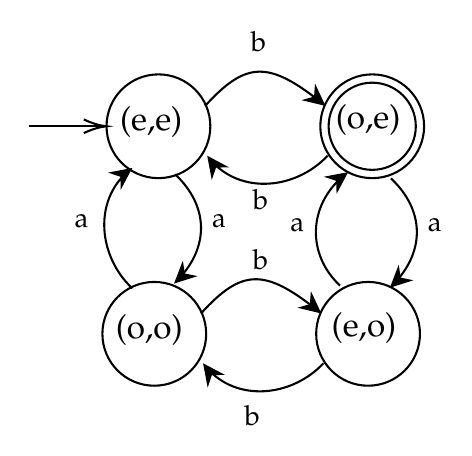
\begin{tikzpicture}[x=0.75pt,y=0.75pt,yscale=-1,xscale=1]
%uncomment if require: \path (0,220); %set diagram left start at 0, and has height of 220

%Shape: Circle [id:dp39498400619483975] 
\draw   (58,62) .. controls (58,48.19) and (69.19,37) .. (83,37) .. controls (96.81,37) and (108,48.19) .. (108,62) .. controls (108,75.81) and (96.81,87) .. (83,87) .. controls (69.19,87) and (58,75.81) .. (58,62) -- cycle ;
%Shape: Circle [id:dp9010152522377439] 
\draw   (165,62) .. controls (165,50.4) and (174.4,41) .. (186,41) .. controls (197.6,41) and (207,50.4) .. (207,62) .. controls (207,73.6) and (197.6,83) .. (186,83) .. controls (174.4,83) and (165,73.6) .. (165,62) -- cycle ;
%Shape: Circle [id:dp9912287585688047] 
\draw   (161,62) .. controls (161,48.19) and (172.19,37) .. (186,37) .. controls (199.81,37) and (211,48.19) .. (211,62) .. controls (211,75.81) and (199.81,87) .. (186,87) .. controls (172.19,87) and (161,75.81) .. (161,62) -- cycle ;
%Curve Lines [id:da5821614928450025] 
\draw    (105.5,52.2) .. controls (125,30.75) and (135.94,30.21) .. (161.5,50.59) ;
\draw [shift={(163.5,52.2)}, rotate = 219.17000000000002] [fill={rgb, 255:red, 0; green, 0; blue, 0 }  ][line width=0.08]  [draw opacity=0] (10.72,-5.15) -- (0,0) -- (10.72,5.15) -- (7.12,0) -- cycle    ;
%Straight Lines [id:da34778597287566804] 
\draw    (20.5,62) -- (56,62) ;
\draw [shift={(58,62)}, rotate = 180] [color={rgb, 255:red, 0; green, 0; blue, 0 }  ][line width=0.75]    (10.93,-3.29) .. controls (6.95,-1.4) and (3.31,-0.3) .. (0,0) .. controls (3.31,0.3) and (6.95,1.4) .. (10.93,3.29)   ;
%Curve Lines [id:da6217387552673006] 
\draw    (164.5,76.2) .. controls (149.14,92.52) and (122.72,95.02) .. (108.25,78.38) ;
\draw [shift={(106.5,76.2)}, rotate = 413.62] [fill={rgb, 255:red, 0; green, 0; blue, 0 }  ][line width=0.08]  [draw opacity=0] (10.72,-5.15) -- (0,0) -- (10.72,5.15) -- (7.12,0) -- cycle    ;
%Shape: Circle [id:dp9208560796051215] 
\draw   (56,162) .. controls (56,148.19) and (67.19,137) .. (81,137) .. controls (94.81,137) and (106,148.19) .. (106,162) .. controls (106,175.81) and (94.81,187) .. (81,187) .. controls (67.19,187) and (56,175.81) .. (56,162) -- cycle ;
%Shape: Circle [id:dp8235560811959559] 
\draw   (159,162) .. controls (159,148.19) and (170.19,137) .. (184,137) .. controls (197.81,137) and (209,148.19) .. (209,162) .. controls (209,175.81) and (197.81,187) .. (184,187) .. controls (170.19,187) and (159,175.81) .. (159,162) -- cycle ;
%Curve Lines [id:da6500653532634744] 
\draw    (103.5,152.2) .. controls (123,130.75) and (133.94,130.21) .. (159.5,150.59) ;
\draw [shift={(161.5,152.2)}, rotate = 219.17000000000002] [fill={rgb, 255:red, 0; green, 0; blue, 0 }  ][line width=0.08]  [draw opacity=0] (10.72,-5.15) -- (0,0) -- (10.72,5.15) -- (7.12,0) -- cycle    ;
%Curve Lines [id:da7930051981173105] 
\draw    (162.5,176.2) .. controls (147.14,192.52) and (120.72,195.02) .. (106.25,178.38) ;
\draw [shift={(104.5,176.2)}, rotate = 413.62] [fill={rgb, 255:red, 0; green, 0; blue, 0 }  ][line width=0.08]  [draw opacity=0] (10.72,-5.15) -- (0,0) -- (10.72,5.15) -- (7.12,0) -- cycle    ;
%Curve Lines [id:da22579429372233273] 
\draw    (70.4,140.1) .. controls (54.08,124.74) and (51.58,98.32) .. (68.22,83.85) ;
\draw [shift={(70.4,82.1)}, rotate = 503.62] [fill={rgb, 255:red, 0; green, 0; blue, 0 }  ][line width=0.08]  [draw opacity=0] (10.72,-5.15) -- (0,0) -- (10.72,5.15) -- (7.12,0) -- cycle    ;
%Curve Lines [id:da7876423213295434] 
\draw    (91.01,85.1) .. controls (107.33,100.46) and (107.51,120.15) .. (92.46,135.86) ;
\draw [shift={(90.5,137.8)}, rotate = 316.74] [fill={rgb, 255:red, 0; green, 0; blue, 0 }  ][line width=0.08]  [draw opacity=0] (10.72,-5.15) -- (0,0) -- (10.72,5.15) -- (7.12,0) -- cycle    ;
%Curve Lines [id:da33701112181486614] 
\draw    (170.5,138.8) .. controls (154.18,123.44) and (155.28,100.06) .. (172.2,85.83) ;
\draw [shift={(174.4,84.1)}, rotate = 503.62] [fill={rgb, 255:red, 0; green, 0; blue, 0 }  ][line width=0.08]  [draw opacity=0] (10.72,-5.15) -- (0,0) -- (10.72,5.15) -- (7.12,0) -- cycle    ;
%Curve Lines [id:da5428522776639717] 
\draw    (195.01,87.1) .. controls (211.33,102.46) and (211.51,122.15) .. (196.46,137.86) ;
\draw [shift={(194.5,139.8)}, rotate = 316.74] [fill={rgb, 255:red, 0; green, 0; blue, 0 }  ][line width=0.08]  [draw opacity=0] (10.72,-5.15) -- (0,0) -- (10.72,5.15) -- (7.12,0) -- cycle    ;

% Text Node
\draw (63,51) node [anchor=north west][inner sep=0.75pt]  [font=\large] [align=left] {(e,e)};
% Text Node
\draw (167,50) node [anchor=north west][inner sep=0.75pt]  [font=\large] [align=left] {(o,e)};
% Text Node
\draw (126,15) node [anchor=north west][inner sep=0.75pt]   [align=left] {b};
% Text Node
\draw (127,91) node [anchor=north west][inner sep=0.75pt]   [align=left] {b};
% Text Node
\draw (61,151) node [anchor=north west][inner sep=0.75pt]  [font=\large] [align=left] {(o,o)};
% Text Node
\draw (165,150) node [anchor=north west][inner sep=0.75pt]  [font=\large] [align=left] {(e,o)};
% Text Node
\draw (127,120) node [anchor=north west][inner sep=0.75pt]   [align=left] {b};
% Text Node
\draw (123,195) node [anchor=north west][inner sep=0.75pt]   [align=left] {b};
% Text Node
\draw (41.17,103.06) node [anchor=north west][inner sep=0.75pt]  [rotate=-0.48] [align=left] {a};
% Text Node
\draw (107.32,103.1) node [anchor=north west][inner sep=0.75pt]  [rotate=-0.02] [align=left] {a};
% Text Node
\draw (145.17,105.06) node [anchor=north west][inner sep=0.75pt]  [rotate=-0.48] [align=left] {a};
% Text Node
\draw (211.32,105.1) node [anchor=north west][inner sep=0.75pt]  [rotate=-0.02] [align=left] {a};


\end{tikzpicture}

where each state is an ordered pair $(q_1, q_2)$ such that $q_1 \in \{e, o\}$ and $q_2 \in \{e, o\}$. 
$q_1$ represents the length of the string (whether even or odd), and 
$q_2$ represents the number of $a$'s, whether even or odd.

\end{enumerate}

\newpage

\begin{prob}\end{prob}

\begin{enumerate}[label=(\alph*)]

\item
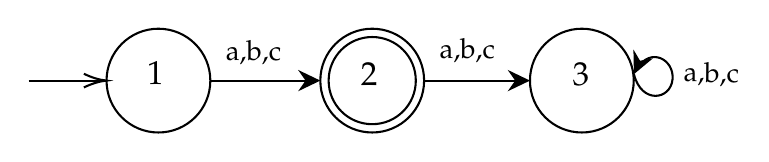
\begin{tikzpicture}[x=0.75pt,y=0.75pt,yscale=-1,xscale=1]
%uncomment if require: \path (0,109); %set diagram left start at 0, and has height of 109

%Shape: Circle [id:dp7434968898937344] 
\draw   (61,48) .. controls (61,34.19) and (72.19,23) .. (86,23) .. controls (99.81,23) and (111,34.19) .. (111,48) .. controls (111,61.81) and (99.81,73) .. (86,73) .. controls (72.19,73) and (61,61.81) .. (61,48) -- cycle ;
%Shape: Circle [id:dp5621109942283065] 
\draw   (168,48) .. controls (168,36.4) and (177.4,27) .. (189,27) .. controls (200.6,27) and (210,36.4) .. (210,48) .. controls (210,59.6) and (200.6,69) .. (189,69) .. controls (177.4,69) and (168,59.6) .. (168,48) -- cycle ;
%Shape: Circle [id:dp4433706105699713] 
\draw   (164,48) .. controls (164,34.19) and (175.19,23) .. (189,23) .. controls (202.81,23) and (214,34.19) .. (214,48) .. controls (214,61.81) and (202.81,73) .. (189,73) .. controls (175.19,73) and (164,61.81) .. (164,48) -- cycle ;
%Straight Lines [id:da78547209217645] 
\draw    (23.5,48) -- (59,48) ;
\draw [shift={(61,48)}, rotate = 180] [color={rgb, 255:red, 0; green, 0; blue, 0 }  ][line width=0.75]    (10.93,-3.29) .. controls (6.95,-1.4) and (3.31,-0.3) .. (0,0) .. controls (3.31,0.3) and (6.95,1.4) .. (10.93,3.29)   ;
%Shape: Circle [id:dp923442747077641] 
\draw   (265,48) .. controls (265,34.19) and (276.19,23) .. (290,23) .. controls (303.81,23) and (315,34.19) .. (315,48) .. controls (315,61.81) and (303.81,73) .. (290,73) .. controls (276.19,73) and (265,61.81) .. (265,48) -- cycle ;
%Curve Lines [id:da3804458806358688] 
\draw    (315.09,44.91) .. controls (318.69,59.41) and (332.69,57.41) .. (333.69,47.41) .. controls (334.62,38.06) and (323.32,31.34) .. (316.45,42.35) ;
\draw [shift={(315.09,44.91)}, rotate = 294.47] [fill={rgb, 255:red, 0; green, 0; blue, 0 }  ][line width=0.08]  [draw opacity=0] (10.72,-5.15) -- (0,0) -- (10.72,5.15) -- (7.12,0) -- cycle    ;
%Straight Lines [id:da1787734768137763] 
\draw    (111,48) -- (161,48) ;
\draw [shift={(164,48)}, rotate = 180] [fill={rgb, 255:red, 0; green, 0; blue, 0 }  ][line width=0.08]  [draw opacity=0] (10.72,-5.15) -- (0,0) -- (10.72,5.15) -- (7.12,0) -- cycle    ;
%Straight Lines [id:da6967311923786783] 
\draw    (214,48) -- (262,48) ;
\draw [shift={(265,48)}, rotate = 180] [fill={rgb, 255:red, 0; green, 0; blue, 0 }  ][line width=0.08]  [draw opacity=0] (10.72,-5.15) -- (0,0) -- (10.72,5.15) -- (7.12,0) -- cycle    ;

% Text Node
\draw (79,37) node [anchor=north west][inner sep=0.75pt]  [font=\large] [align=left] {1};
% Text Node
\draw (182,38) node [anchor=north west][inner sep=0.75pt]  [font=\large] [align=left] {2};
% Text Node
\draw (117,27) node [anchor=north west][inner sep=0.75pt]   [align=left] {a,b,c};
% Text Node
\draw (220,26) node [anchor=north west][inner sep=0.75pt]   [align=left] {a,b,c};
% Text Node
\draw (337.66,37.37) node [anchor=north west][inner sep=0.75pt]  [rotate=-0.49] [align=left] {a,b,c};
% Text Node
\draw (284,38) node [anchor=north west][inner sep=0.75pt]  [font=\large] [align=left] {3};


\end{tikzpicture}

where 1 is the inital state, and 2 is a state where its a single letter $a$, $b$, or $c$, and 3 
is a rejected state where we've exceeded the one-letter limit.

\item
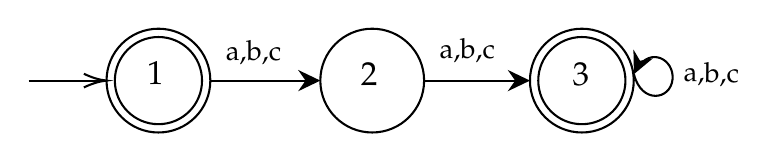
\begin{tikzpicture}[x=0.75pt,y=0.75pt,yscale=-1,xscale=1]
%uncomment if require: \path (0,83); %set diagram left start at 0, and has height of 83

%Shape: Circle [id:dp9085606646795719] 
\draw   (65,47) .. controls (65,33.19) and (76.19,22) .. (90,22) .. controls (103.81,22) and (115,33.19) .. (115,47) .. controls (115,60.81) and (103.81,72) .. (90,72) .. controls (76.19,72) and (65,60.81) .. (65,47) -- cycle ;
%Shape: Circle [id:dp7724236271883884] 
\draw   (69,47) .. controls (69,35.4) and (78.4,26) .. (90,26) .. controls (101.6,26) and (111,35.4) .. (111,47) .. controls (111,58.6) and (101.6,68) .. (90,68) .. controls (78.4,68) and (69,58.6) .. (69,47) -- cycle ;
%Shape: Circle [id:dp9869729063952344] 
\draw   (168,47) .. controls (168,33.19) and (179.19,22) .. (193,22) .. controls (206.81,22) and (218,33.19) .. (218,47) .. controls (218,60.81) and (206.81,72) .. (193,72) .. controls (179.19,72) and (168,60.81) .. (168,47) -- cycle ;
%Straight Lines [id:da7342861308388684] 
\draw    (27.5,47) -- (63,47) ;
\draw [shift={(65,47)}, rotate = 180] [color={rgb, 255:red, 0; green, 0; blue, 0 }  ][line width=0.75]    (10.93,-3.29) .. controls (6.95,-1.4) and (3.31,-0.3) .. (0,0) .. controls (3.31,0.3) and (6.95,1.4) .. (10.93,3.29)   ;
%Shape: Circle [id:dp8101622500517194] 
\draw   (269,47) .. controls (269,33.19) and (280.19,22) .. (294,22) .. controls (307.81,22) and (319,33.19) .. (319,47) .. controls (319,60.81) and (307.81,72) .. (294,72) .. controls (280.19,72) and (269,60.81) .. (269,47) -- cycle ;
%Curve Lines [id:da14872349722721245] 
\draw    (319.09,43.91) .. controls (322.69,58.41) and (336.69,56.41) .. (337.69,46.41) .. controls (338.62,37.06) and (327.32,30.34) .. (320.45,41.35) ;
\draw [shift={(319.09,43.91)}, rotate = 294.47] [fill={rgb, 255:red, 0; green, 0; blue, 0 }  ][line width=0.08]  [draw opacity=0] (10.72,-5.15) -- (0,0) -- (10.72,5.15) -- (7.12,0) -- cycle    ;
%Straight Lines [id:da05312994054050879] 
\draw    (115,47) -- (165,47) ;
\draw [shift={(168,47)}, rotate = 180] [fill={rgb, 255:red, 0; green, 0; blue, 0 }  ][line width=0.08]  [draw opacity=0] (10.72,-5.15) -- (0,0) -- (10.72,5.15) -- (7.12,0) -- cycle    ;
%Straight Lines [id:da42538228977102954] 
\draw    (218,47) -- (266,47) ;
\draw [shift={(269,47)}, rotate = 180] [fill={rgb, 255:red, 0; green, 0; blue, 0 }  ][line width=0.08]  [draw opacity=0] (10.72,-5.15) -- (0,0) -- (10.72,5.15) -- (7.12,0) -- cycle    ;
%Shape: Circle [id:dp1180280870023187] 
\draw   (273,47) .. controls (273,35.4) and (282.4,26) .. (294,26) .. controls (305.6,26) and (315,35.4) .. (315,47) .. controls (315,58.6) and (305.6,68) .. (294,68) .. controls (282.4,68) and (273,58.6) .. (273,47) -- cycle ;

% Text Node
\draw (83,36) node [anchor=north west][inner sep=0.75pt]  [font=\large] [align=left] {1};
% Text Node
\draw (186,37) node [anchor=north west][inner sep=0.75pt]  [font=\large] [align=left] {2};
% Text Node
\draw (121,26) node [anchor=north west][inner sep=0.75pt]   [align=left] {a,b,c};
% Text Node
\draw (224,25) node [anchor=north west][inner sep=0.75pt]   [align=left] {a,b,c};
% Text Node
\draw (341.66,36.37) node [anchor=north west][inner sep=0.75pt]  [rotate=-0.49] [align=left] {a,b,c};
% Text Node
\draw (288,37) node [anchor=north west][inner sep=0.75pt]  [font=\large] [align=left] {3};


\end{tikzpicture}

where 1 is the initial state, and 2 is a state where it is a single letter $a$, $b$, or $c$. 3 is 
an accepting state where our word is not simply a single letter.

\end{enumerate}

\begin{prob}\end{prob}

Diagram and numbered for explanations down below. \\

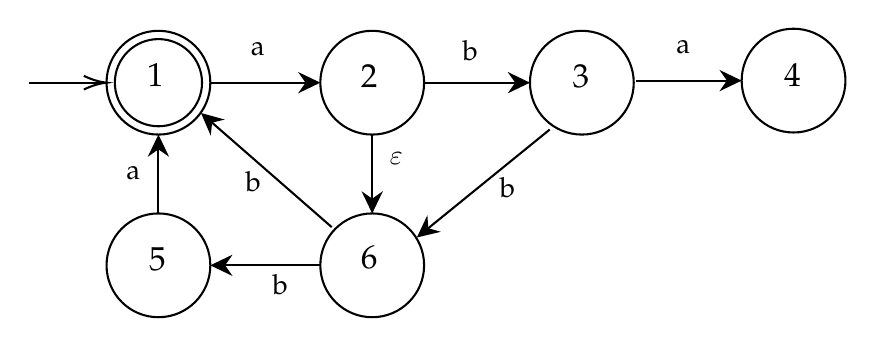
\begin{tikzpicture}[x=0.75pt,y=0.75pt,yscale=-1,xscale=1]
%uncomment if require: \path (0,181); %set diagram left start at 0, and has height of 181

%Shape: Circle [id:dp5215305385073898] 
\draw   (66,48) .. controls (66,34.19) and (77.19,23) .. (91,23) .. controls (104.81,23) and (116,34.19) .. (116,48) .. controls (116,61.81) and (104.81,73) .. (91,73) .. controls (77.19,73) and (66,61.81) .. (66,48) -- cycle ;
%Shape: Circle [id:dp5602906042350988] 
\draw   (70,48) .. controls (70,36.4) and (79.4,27) .. (91,27) .. controls (102.6,27) and (112,36.4) .. (112,48) .. controls (112,59.6) and (102.6,69) .. (91,69) .. controls (79.4,69) and (70,59.6) .. (70,48) -- cycle ;
%Shape: Circle [id:dp5077824048097472] 
\draw   (169,48) .. controls (169,34.19) and (180.19,23) .. (194,23) .. controls (207.81,23) and (219,34.19) .. (219,48) .. controls (219,61.81) and (207.81,73) .. (194,73) .. controls (180.19,73) and (169,61.81) .. (169,48) -- cycle ;
%Straight Lines [id:da36578110754431226] 
\draw    (28.5,48) -- (64,48) ;
\draw [shift={(66,48)}, rotate = 180] [color={rgb, 255:red, 0; green, 0; blue, 0 }  ][line width=0.75]    (10.93,-3.29) .. controls (6.95,-1.4) and (3.31,-0.3) .. (0,0) .. controls (3.31,0.3) and (6.95,1.4) .. (10.93,3.29)   ;
%Shape: Circle [id:dp12089094644585452] 
\draw   (270,48) .. controls (270,34.19) and (281.19,23) .. (295,23) .. controls (308.81,23) and (320,34.19) .. (320,48) .. controls (320,61.81) and (308.81,73) .. (295,73) .. controls (281.19,73) and (270,61.81) .. (270,48) -- cycle ;
%Straight Lines [id:da6501578343120367] 
\draw    (116,48) -- (166,48) ;
\draw [shift={(169,48)}, rotate = 180] [fill={rgb, 255:red, 0; green, 0; blue, 0 }  ][line width=0.08]  [draw opacity=0] (10.72,-5.15) -- (0,0) -- (10.72,5.15) -- (7.12,0) -- cycle    ;
%Straight Lines [id:da5897171188999353] 
\draw    (219,48) -- (267,48) ;
\draw [shift={(270,48)}, rotate = 180] [fill={rgb, 255:red, 0; green, 0; blue, 0 }  ][line width=0.08]  [draw opacity=0] (10.72,-5.15) -- (0,0) -- (10.72,5.15) -- (7.12,0) -- cycle    ;
%Shape: Circle [id:dp20377815134473898] 
\draw   (372,47) .. controls (372,33.19) and (383.19,22) .. (397,22) .. controls (410.81,22) and (422,33.19) .. (422,47) .. controls (422,60.81) and (410.81,72) .. (397,72) .. controls (383.19,72) and (372,60.81) .. (372,47) -- cycle ;
%Straight Lines [id:da18754139349267152] 
\draw    (321,47) -- (369,47) ;
\draw [shift={(372,47)}, rotate = 180] [fill={rgb, 255:red, 0; green, 0; blue, 0 }  ][line width=0.08]  [draw opacity=0] (10.72,-5.15) -- (0,0) -- (10.72,5.15) -- (7.12,0) -- cycle    ;
%Shape: Circle [id:dp8892361837808249] 
\draw   (66,136) .. controls (66,122.19) and (77.19,111) .. (91,111) .. controls (104.81,111) and (116,122.19) .. (116,136) .. controls (116,149.81) and (104.81,161) .. (91,161) .. controls (77.19,161) and (66,149.81) .. (66,136) -- cycle ;
%Shape: Circle [id:dp6597683311622633] 
\draw   (169,136) .. controls (169,122.19) and (180.19,111) .. (194,111) .. controls (207.81,111) and (219,122.19) .. (219,136) .. controls (219,149.81) and (207.81,161) .. (194,161) .. controls (180.19,161) and (169,149.81) .. (169,136) -- cycle ;
%Straight Lines [id:da3108361676167437] 
\draw    (91,111) -- (91,76) ;
\draw [shift={(91,73)}, rotate = 450] [fill={rgb, 255:red, 0; green, 0; blue, 0 }  ][line width=0.08]  [draw opacity=0] (10.72,-5.15) -- (0,0) -- (10.72,5.15) -- (7.12,0) -- cycle    ;
%Straight Lines [id:da4336120168262514] 
\draw    (194,73) -- (194,108) ;
\draw [shift={(194,111)}, rotate = 270] [fill={rgb, 255:red, 0; green, 0; blue, 0 }  ][line width=0.08]  [draw opacity=0] (10.72,-5.15) -- (0,0) -- (10.72,5.15) -- (7.12,0) -- cycle    ;
%Straight Lines [id:da9285909422329612] 
\draw    (169,136) -- (119,136) ;
\draw [shift={(116,136)}, rotate = 360] [fill={rgb, 255:red, 0; green, 0; blue, 0 }  ][line width=0.08]  [draw opacity=0] (10.72,-5.15) -- (0,0) -- (10.72,5.15) -- (7.12,0) -- cycle    ;
%Straight Lines [id:da033530180567733714] 
\draw    (174.5,117.6) -- (113.76,64.57) ;
\draw [shift={(111.5,62.6)}, rotate = 401.12] [fill={rgb, 255:red, 0; green, 0; blue, 0 }  ][line width=0.08]  [draw opacity=0] (10.72,-5.15) -- (0,0) -- (10.72,5.15) -- (7.12,0) -- cycle    ;
%Straight Lines [id:da6579247517790194] 
\draw    (279.5,70.6) -- (217.83,120.71) ;
\draw [shift={(215.5,122.6)}, rotate = 320.90999999999997] [fill={rgb, 255:red, 0; green, 0; blue, 0 }  ][line width=0.08]  [draw opacity=0] (10.72,-5.15) -- (0,0) -- (10.72,5.15) -- (7.12,0) -- cycle    ;

% Text Node
\draw (84,37) node [anchor=north west][inner sep=0.75pt]  [font=\large] [align=left] {1};
% Text Node
\draw (187,38) node [anchor=north west][inner sep=0.75pt]  [font=\large] [align=left] {2};
% Text Node
\draw (134,27) node [anchor=north west][inner sep=0.75pt]   [align=left] {a};
% Text Node
\draw (236,26) node [anchor=north west][inner sep=0.75pt]   [align=left] {b};
% Text Node
\draw (289,38) node [anchor=north west][inner sep=0.75pt]  [font=\large] [align=left] {3};
% Text Node
\draw (391,37) node [anchor=north west][inner sep=0.75pt]  [font=\large] [align=left] {4};
% Text Node
\draw (339,26) node [anchor=north west][inner sep=0.75pt]   [align=left] {a};
% Text Node
\draw (85,126) node [anchor=north west][inner sep=0.75pt]  [font=\large] [align=left] {5};
% Text Node
\draw (187,125) node [anchor=north west][inner sep=0.75pt]  [font=\large] [align=left] {6};
% Text Node
\draw (201,80) node [anchor=north west][inner sep=0.75pt]   [align=left] {$\displaystyle \varepsilon $};
% Text Node
\draw (74,87) node [anchor=north west][inner sep=0.75pt]   [align=left] {a};
% Text Node
\draw (144.5,139) node [anchor=north west][inner sep=0.75pt]   [align=left] {b};
% Text Node
\draw (131.5,89) node [anchor=north west][inner sep=0.75pt]   [align=left] {b};
% Text Node
\draw (254,92) node [anchor=north west][inner sep=0.75pt]   [align=left] {b};


\end{tikzpicture}

\begin{enumerate}[label=(\alph*)]

\item
$aa$ is not accepted, because the first $a$ can take us from 1 $\rightarrow$ 2 $\rightarrow$ 6, but from there we are stuck without a $b$.

\item
$aba$ is accepted, because we can go 1 $\rightarrow$ 2 $\rightarrow$ 6 $\rightarrow$ 5 $\rightarrow$ 1.

\item
$abb$ is not accepted, because the first $a$ can take us to 2 or 6, but from there, we cannot get back to 1 with 2 $b$'s. 
Going 6 $\rightarrow$ 5 needs an $a$, 6 $\rightarrow$ 1 $\rightarrow$ $\varnothing$ is not accepted, 
2 $\rightarrow$ 3 $\rightarrow$ 6 is also not accepting.

\item
$ab$ is accepted, because we can go 1 $\rightarrow$ 2 $\rightarrow$ 6 $\rightarrow$ 1.

\item
$abab$ is accepted, because we can go 1 $\rightarrow$ 2 $\rightarrow$ 6 $\rightarrow$ 1 $\rightarrow$ 2 $\rightarrow$ 6 $\rightarrow$ 1.

\end{enumerate}

\newpage

\begin{prob}\end{prob}

$L = \{ w \hspace{1px} | \hspace{1px} w = \text{ starts with a followed by 1-3 b's } \hspace{1px} \text{OR} \hspace{1px} w = bbb \}$ 

\begin{prob}\end{prob}

\begin{enumerate}[label=(\alph*)]

\item
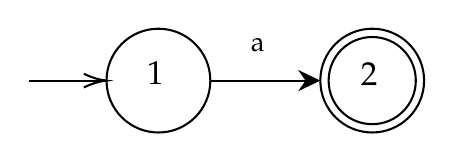
\begin{tikzpicture}[x=0.75pt,y=0.75pt,yscale=-1,xscale=1]
%uncomment if require: \path (0,92); %set diagram left start at 0, and has height of 92

%Shape: Circle [id:dp015975736039515853] 
\draw   (69,48) .. controls (69,34.19) and (80.19,23) .. (94,23) .. controls (107.81,23) and (119,34.19) .. (119,48) .. controls (119,61.81) and (107.81,73) .. (94,73) .. controls (80.19,73) and (69,61.81) .. (69,48) -- cycle ;
%Shape: Circle [id:dp8467337287246317] 
\draw   (176,48) .. controls (176,36.4) and (185.4,27) .. (197,27) .. controls (208.6,27) and (218,36.4) .. (218,48) .. controls (218,59.6) and (208.6,69) .. (197,69) .. controls (185.4,69) and (176,59.6) .. (176,48) -- cycle ;
%Shape: Circle [id:dp8507566475858015] 
\draw   (172,48) .. controls (172,34.19) and (183.19,23) .. (197,23) .. controls (210.81,23) and (222,34.19) .. (222,48) .. controls (222,61.81) and (210.81,73) .. (197,73) .. controls (183.19,73) and (172,61.81) .. (172,48) -- cycle ;
%Straight Lines [id:da3483027630188973] 
\draw    (31.5,48) -- (67,48) ;
\draw [shift={(69,48)}, rotate = 180] [color={rgb, 255:red, 0; green, 0; blue, 0 }  ][line width=0.75]    (10.93,-3.29) .. controls (6.95,-1.4) and (3.31,-0.3) .. (0,0) .. controls (3.31,0.3) and (6.95,1.4) .. (10.93,3.29)   ;
%Straight Lines [id:da5692271074984843] 
\draw    (119,48) -- (169,48) ;
\draw [shift={(172,48)}, rotate = 180] [fill={rgb, 255:red, 0; green, 0; blue, 0 }  ][line width=0.08]  [draw opacity=0] (10.72,-5.15) -- (0,0) -- (10.72,5.15) -- (7.12,0) -- cycle    ;

% Text Node
\draw (87,37) node [anchor=north west][inner sep=0.75pt]  [font=\large] [align=left] {1};
% Text Node
\draw (190,38) node [anchor=north west][inner sep=0.75pt]  [font=\large] [align=left] {2};
% Text Node
\draw (137,26) node [anchor=north west][inner sep=0.75pt]   [align=left] {a};


\end{tikzpicture}

\item
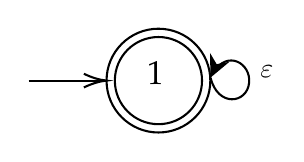
\begin{tikzpicture}[x=0.75pt,y=0.75pt,yscale=-1,xscale=1]
%uncomment if require: \path (0,72); %set diagram left start at 0, and has height of 72

%Shape: Circle [id:dp7612884103952993] 
\draw   (65,39) .. controls (65,25.19) and (76.19,14) .. (90,14) .. controls (103.81,14) and (115,25.19) .. (115,39) .. controls (115,52.81) and (103.81,64) .. (90,64) .. controls (76.19,64) and (65,52.81) .. (65,39) -- cycle ;
%Straight Lines [id:da5146020690255284] 
\draw    (27.5,39) -- (63,39) ;
\draw [shift={(65,39)}, rotate = 180] [color={rgb, 255:red, 0; green, 0; blue, 0 }  ][line width=0.75]    (10.93,-3.29) .. controls (6.95,-1.4) and (3.31,-0.3) .. (0,0) .. controls (3.31,0.3) and (6.95,1.4) .. (10.93,3.29)   ;
%Shape: Circle [id:dp21510562029190683] 
\draw   (69,39) .. controls (69,27.4) and (78.4,18) .. (90,18) .. controls (101.6,18) and (111,27.4) .. (111,39) .. controls (111,50.6) and (101.6,60) .. (90,60) .. controls (78.4,60) and (69,50.6) .. (69,39) -- cycle ;
%Curve Lines [id:da40282050866144425] 
\draw    (115.09,37.56) .. controls (118.69,52.06) and (132.69,50.06) .. (133.69,40.06) .. controls (134.62,30.71) and (123.32,23.98) .. (116.45,35) ;
\draw [shift={(115.09,37.56)}, rotate = 294.47] [fill={rgb, 255:red, 0; green, 0; blue, 0 }  ][line width=0.08]  [draw opacity=0] (10.72,-5.15) -- (0,0) -- (10.72,5.15) -- (7.12,0) -- cycle    ;

% Text Node
\draw (83,28) node [anchor=north west][inner sep=0.75pt]  [font=\large] [align=left] {1};
% Text Node
\draw (137.66,30.02) node [anchor=north west][inner sep=0.75pt]  [rotate=-0.49] [align=left] {$\displaystyle \varepsilon $};


\end{tikzpicture}

\item
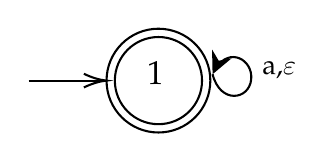
\begin{tikzpicture}[x=0.75pt,y=0.75pt,yscale=-1,xscale=1]
%uncomment if require: \path (0,93); %set diagram left start at 0, and has height of 93

%Shape: Circle [id:dp619134690418123] 
\draw   (64,46) .. controls (64,32.19) and (75.19,21) .. (89,21) .. controls (102.81,21) and (114,32.19) .. (114,46) .. controls (114,59.81) and (102.81,71) .. (89,71) .. controls (75.19,71) and (64,59.81) .. (64,46) -- cycle ;
%Straight Lines [id:da06564898950998943] 
\draw    (26.5,46) -- (62,46) ;
\draw [shift={(64,46)}, rotate = 180] [color={rgb, 255:red, 0; green, 0; blue, 0 }  ][line width=0.75]    (10.93,-3.29) .. controls (6.95,-1.4) and (3.31,-0.3) .. (0,0) .. controls (3.31,0.3) and (6.95,1.4) .. (10.93,3.29)   ;
%Curve Lines [id:da5213186338084936] 
\draw    (115.09,42.91) .. controls (118.69,57.41) and (132.69,55.41) .. (133.69,45.41) .. controls (134.62,36.06) and (123.32,29.34) .. (116.45,40.35) ;
\draw [shift={(115.09,42.91)}, rotate = 294.47] [fill={rgb, 255:red, 0; green, 0; blue, 0 }  ][line width=0.08]  [draw opacity=0] (10.72,-5.15) -- (0,0) -- (10.72,5.15) -- (7.12,0) -- cycle    ;
%Shape: Circle [id:dp26774557602448357] 
\draw   (68,46) .. controls (68,34.4) and (77.4,25) .. (89,25) .. controls (100.6,25) and (110,34.4) .. (110,46) .. controls (110,57.6) and (100.6,67) .. (89,67) .. controls (77.4,67) and (68,57.6) .. (68,46) -- cycle ;

% Text Node
\draw (82,35) node [anchor=north west][inner sep=0.75pt]  [font=\large] [align=left] {1};
% Text Node
\draw (137.66,35.37) node [anchor=north west][inner sep=0.75pt]  [rotate=-0.49] [align=left] {a,$\displaystyle \varepsilon $};


\end{tikzpicture}

\item
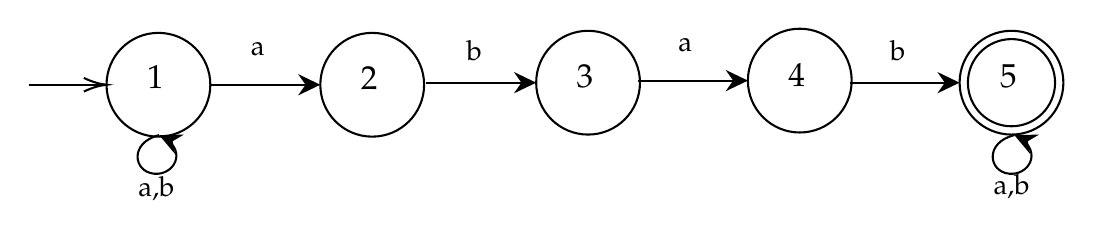
\begin{tikzpicture}[x=0.75pt,y=0.75pt,yscale=-1,xscale=1]
%uncomment if require: \path (0,117); %set diagram left start at 0, and has height of 117

%Shape: Circle [id:dp3639594831559261] 
\draw   (64,46) .. controls (64,32.19) and (75.19,21) .. (89,21) .. controls (102.81,21) and (114,32.19) .. (114,46) .. controls (114,59.81) and (102.81,71) .. (89,71) .. controls (75.19,71) and (64,59.81) .. (64,46) -- cycle ;
%Shape: Circle [id:dp5582441870645005] 
\draw   (167,46) .. controls (167,32.19) and (178.19,21) .. (192,21) .. controls (205.81,21) and (217,32.19) .. (217,46) .. controls (217,59.81) and (205.81,71) .. (192,71) .. controls (178.19,71) and (167,59.81) .. (167,46) -- cycle ;
%Straight Lines [id:da1354789551356177] 
\draw    (26.5,46) -- (62,46) ;
\draw [shift={(64,46)}, rotate = 180] [color={rgb, 255:red, 0; green, 0; blue, 0 }  ][line width=0.75]    (10.93,-3.29) .. controls (6.95,-1.4) and (3.31,-0.3) .. (0,0) .. controls (3.31,0.3) and (6.95,1.4) .. (10.93,3.29)   ;
%Straight Lines [id:da933986218351992] 
\draw    (114,46) -- (164,46) ;
\draw [shift={(167,46)}, rotate = 180] [fill={rgb, 255:red, 0; green, 0; blue, 0 }  ][line width=0.08]  [draw opacity=0] (10.72,-5.15) -- (0,0) -- (10.72,5.15) -- (7.12,0) -- cycle    ;
%Shape: Circle [id:dp41962525049316257] 
\draw   (271,45) .. controls (271,31.19) and (282.19,20) .. (296,20) .. controls (309.81,20) and (321,31.19) .. (321,45) .. controls (321,58.81) and (309.81,70) .. (296,70) .. controls (282.19,70) and (271,58.81) .. (271,45) -- cycle ;
%Straight Lines [id:da2713796983651633] 
\draw    (218,45) -- (268,45) ;
\draw [shift={(271,45)}, rotate = 180] [fill={rgb, 255:red, 0; green, 0; blue, 0 }  ][line width=0.08]  [draw opacity=0] (10.72,-5.15) -- (0,0) -- (10.72,5.15) -- (7.12,0) -- cycle    ;
%Shape: Circle [id:dp19612387490457484] 
\draw   (373,44) .. controls (373,30.19) and (384.19,19) .. (398,19) .. controls (411.81,19) and (423,30.19) .. (423,44) .. controls (423,57.81) and (411.81,69) .. (398,69) .. controls (384.19,69) and (373,57.81) .. (373,44) -- cycle ;
%Straight Lines [id:da035606009119916626] 
\draw    (320,44) -- (370,44) ;
\draw [shift={(373,44)}, rotate = 180] [fill={rgb, 255:red, 0; green, 0; blue, 0 }  ][line width=0.08]  [draw opacity=0] (10.72,-5.15) -- (0,0) -- (10.72,5.15) -- (7.12,0) -- cycle    ;
%Shape: Circle [id:dp5913384099541268] 
\draw   (475,45) .. controls (475,31.19) and (486.19,20) .. (500,20) .. controls (513.81,20) and (525,31.19) .. (525,45) .. controls (525,58.81) and (513.81,70) .. (500,70) .. controls (486.19,70) and (475,58.81) .. (475,45) -- cycle ;
%Straight Lines [id:da8939147402411887] 
\draw    (422,45) -- (472,45) ;
\draw [shift={(475,45)}, rotate = 180] [fill={rgb, 255:red, 0; green, 0; blue, 0 }  ][line width=0.08]  [draw opacity=0] (10.72,-5.15) -- (0,0) -- (10.72,5.15) -- (7.12,0) -- cycle    ;
%Shape: Circle [id:dp9603499922693886] 
\draw   (479,45) .. controls (479,33.4) and (488.4,24) .. (500,24) .. controls (511.6,24) and (521,33.4) .. (521,45) .. controls (521,56.6) and (511.6,66) .. (500,66) .. controls (488.4,66) and (479,56.6) .. (479,45) -- cycle ;
%Curve Lines [id:da04375911820028855] 
\draw    (89.38,70.26) .. controls (74.88,73.86) and (76.88,87.86) .. (86.88,88.86) .. controls (96.23,89.8) and (102.96,78.5) .. (91.94,71.63) ;
\draw [shift={(89.38,70.26)}, rotate = 384.47] [fill={rgb, 255:red, 0; green, 0; blue, 0 }  ][line width=0.08]  [draw opacity=0] (10.72,-5.15) -- (0,0) -- (10.72,5.15) -- (7.12,0) -- cycle    ;
%Curve Lines [id:da09688212447072031] 
\draw    (501.38,70.26) .. controls (486.88,73.86) and (488.88,87.86) .. (498.88,88.86) .. controls (508.23,89.8) and (514.96,78.5) .. (503.94,71.63) ;
\draw [shift={(501.38,70.26)}, rotate = 384.47] [fill={rgb, 255:red, 0; green, 0; blue, 0 }  ][line width=0.08]  [draw opacity=0] (10.72,-5.15) -- (0,0) -- (10.72,5.15) -- (7.12,0) -- cycle    ;

% Text Node
\draw (82,35) node [anchor=north west][inner sep=0.75pt]  [font=\large] [align=left] {1};
% Text Node
\draw (185,36) node [anchor=north west][inner sep=0.75pt]  [font=\large] [align=left] {2};
% Text Node
\draw (132,24) node [anchor=north west][inner sep=0.75pt]   [align=left] {a};
% Text Node
\draw (289,35) node [anchor=north west][inner sep=0.75pt]  [font=\large] [align=left] {3};
% Text Node
\draw (236,23) node [anchor=north west][inner sep=0.75pt]   [align=left] {b};
% Text Node
\draw (391,34) node [anchor=north west][inner sep=0.75pt]  [font=\large] [align=left] {4};
% Text Node
\draw (338,22) node [anchor=north west][inner sep=0.75pt]   [align=left] {a};
% Text Node
\draw (493,35) node [anchor=north west][inner sep=0.75pt]  [font=\large] [align=left] {5};
% Text Node
\draw (440,23) node [anchor=north west][inner sep=0.75pt]   [align=left] {b};
% Text Node
\draw (77.88,88.76) node [anchor=north west][inner sep=0.75pt]   [align=left] {a,b};
% Text Node
\draw (489.88,87.76) node [anchor=north west][inner sep=0.75pt]   [align=left] {a,b};


\end{tikzpicture}

\item
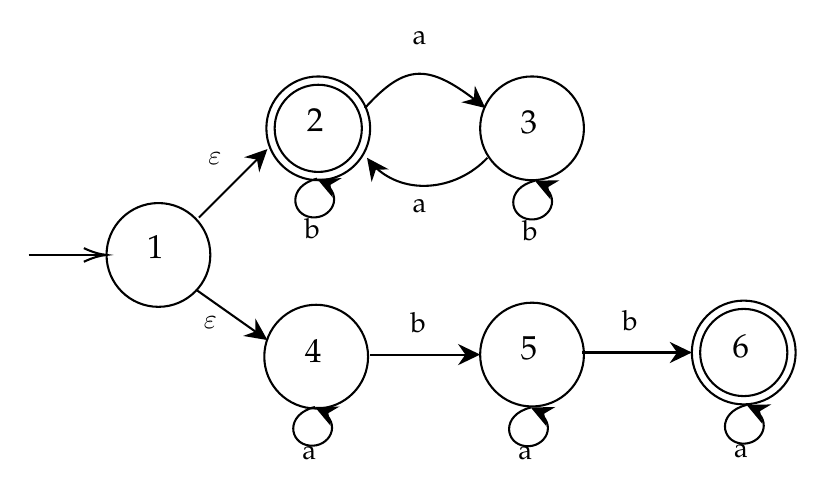
\begin{tikzpicture}[x=0.75pt,y=0.75pt,yscale=-1,xscale=1]
%uncomment if require: \path (0,252); %set diagram left start at 0, and has height of 252

%Shape: Circle [id:dp9580070785476751] 
\draw   (185,70) .. controls (185,56.19) and (196.19,45) .. (210,45) .. controls (223.81,45) and (235,56.19) .. (235,70) .. controls (235,83.81) and (223.81,95) .. (210,95) .. controls (196.19,95) and (185,83.81) .. (185,70) -- cycle ;
%Shape: Circle [id:dp6481599160987115] 
\draw   (189,70) .. controls (189,58.4) and (198.4,49) .. (210,49) .. controls (221.6,49) and (231,58.4) .. (231,70) .. controls (231,81.6) and (221.6,91) .. (210,91) .. controls (198.4,91) and (189,81.6) .. (189,70) -- cycle ;
%Shape: Circle [id:dp4804105955084119] 
\draw   (288,70) .. controls (288,56.19) and (299.19,45) .. (313,45) .. controls (326.81,45) and (338,56.19) .. (338,70) .. controls (338,83.81) and (326.81,95) .. (313,95) .. controls (299.19,95) and (288,83.81) .. (288,70) -- cycle ;
%Curve Lines [id:da5143406822940446] 
\draw    (232.5,60.2) .. controls (252,38.75) and (262.94,38.21) .. (288.5,58.59) ;
\draw [shift={(290.5,60.2)}, rotate = 219.17000000000002] [fill={rgb, 255:red, 0; green, 0; blue, 0 }  ][line width=0.08]  [draw opacity=0] (10.72,-5.15) -- (0,0) -- (10.72,5.15) -- (7.12,0) -- cycle    ;
%Curve Lines [id:da12657330613094908] 
\draw    (291.5,84.2) .. controls (276.14,100.52) and (249.72,103.02) .. (235.25,86.38) ;
\draw [shift={(233.5,84.2)}, rotate = 413.62] [fill={rgb, 255:red, 0; green, 0; blue, 0 }  ][line width=0.08]  [draw opacity=0] (10.72,-5.15) -- (0,0) -- (10.72,5.15) -- (7.12,0) -- cycle    ;
%Shape: Circle [id:dp10692847203029077] 
\draw   (184,180) .. controls (184,166.19) and (195.19,155) .. (209,155) .. controls (222.81,155) and (234,166.19) .. (234,180) .. controls (234,193.81) and (222.81,205) .. (209,205) .. controls (195.19,205) and (184,193.81) .. (184,180) -- cycle ;
%Shape: Circle [id:dp028465108381639848] 
\draw   (288,179) .. controls (288,165.19) and (299.19,154) .. (313,154) .. controls (326.81,154) and (338,165.19) .. (338,179) .. controls (338,192.81) and (326.81,204) .. (313,204) .. controls (299.19,204) and (288,192.81) .. (288,179) -- cycle ;
%Straight Lines [id:da8608352841282201] 
\draw    (235,179) -- (285,179) ;
\draw [shift={(288,179)}, rotate = 180] [fill={rgb, 255:red, 0; green, 0; blue, 0 }  ][line width=0.08]  [draw opacity=0] (10.72,-5.15) -- (0,0) -- (10.72,5.15) -- (7.12,0) -- cycle    ;
%Shape: Circle [id:dp0025579760276797092] 
\draw   (390,178) .. controls (390,164.19) and (401.19,153) .. (415,153) .. controls (428.81,153) and (440,164.19) .. (440,178) .. controls (440,191.81) and (428.81,203) .. (415,203) .. controls (401.19,203) and (390,191.81) .. (390,178) -- cycle ;
%Straight Lines [id:da7158805633581309] 
\draw    (337,178) -- (387,178) ;
\draw [shift={(390,178)}, rotate = 180] [fill={rgb, 255:red, 0; green, 0; blue, 0 }  ][line width=0.08]  [draw opacity=0] (10.72,-5.15) -- (0,0) -- (10.72,5.15) -- (7.12,0) -- cycle    ;
%Curve Lines [id:da1552167752818323] 
\draw    (209.38,94.26) .. controls (194.88,97.86) and (196.88,111.86) .. (206.88,112.86) .. controls (216.23,113.8) and (222.96,102.5) .. (211.94,95.63) ;
\draw [shift={(209.38,94.26)}, rotate = 384.47] [fill={rgb, 255:red, 0; green, 0; blue, 0 }  ][line width=0.08]  [draw opacity=0] (10.72,-5.15) -- (0,0) -- (10.72,5.15) -- (7.12,0) -- cycle    ;
%Curve Lines [id:da04300840267948414] 
\draw    (314.38,95.26) .. controls (299.88,98.86) and (301.88,112.86) .. (311.88,113.86) .. controls (321.23,114.8) and (327.96,103.5) .. (316.94,96.63) ;
\draw [shift={(314.38,95.26)}, rotate = 384.47] [fill={rgb, 255:red, 0; green, 0; blue, 0 }  ][line width=0.08]  [draw opacity=0] (10.72,-5.15) -- (0,0) -- (10.72,5.15) -- (7.12,0) -- cycle    ;
%Curve Lines [id:da10572007218563906] 
\draw    (208.38,204.26) .. controls (193.88,207.86) and (195.88,221.86) .. (205.88,222.86) .. controls (215.23,223.8) and (221.96,212.5) .. (210.94,205.63) ;
\draw [shift={(208.38,204.26)}, rotate = 384.47] [fill={rgb, 255:red, 0; green, 0; blue, 0 }  ][line width=0.08]  [draw opacity=0] (10.72,-5.15) -- (0,0) -- (10.72,5.15) -- (7.12,0) -- cycle    ;
%Curve Lines [id:da07427980983404514] 
\draw    (416.38,203.26) .. controls (401.88,206.86) and (403.88,220.86) .. (413.88,221.86) .. controls (423.23,222.8) and (429.96,211.5) .. (418.94,204.63) ;
\draw [shift={(416.38,203.26)}, rotate = 384.47] [fill={rgb, 255:red, 0; green, 0; blue, 0 }  ][line width=0.08]  [draw opacity=0] (10.72,-5.15) -- (0,0) -- (10.72,5.15) -- (7.12,0) -- cycle    ;
%Shape: Circle [id:dp1900534127154747] 
\draw   (394,178) .. controls (394,166.4) and (403.4,157) .. (415,157) .. controls (426.6,157) and (436,166.4) .. (436,178) .. controls (436,189.6) and (426.6,199) .. (415,199) .. controls (403.4,199) and (394,189.6) .. (394,178) -- cycle ;
%Shape: Circle [id:dp3260182564597558] 
\draw   (108,131) .. controls (108,117.19) and (119.19,106) .. (133,106) .. controls (146.81,106) and (158,117.19) .. (158,131) .. controls (158,144.81) and (146.81,156) .. (133,156) .. controls (119.19,156) and (108,144.81) .. (108,131) -- cycle ;
%Straight Lines [id:da1660030301392883] 
\draw    (70.5,131) -- (106,131) ;
\draw [shift={(108,131)}, rotate = 180] [color={rgb, 255:red, 0; green, 0; blue, 0 }  ][line width=0.75]    (10.93,-3.29) .. controls (6.95,-1.4) and (3.31,-0.3) .. (0,0) .. controls (3.31,0.3) and (6.95,1.4) .. (10.93,3.29)   ;
%Straight Lines [id:da6026999077539652] 
\draw    (152.5,113) -- (183.38,82.12) ;
\draw [shift={(185.5,80)}, rotate = 495] [fill={rgb, 255:red, 0; green, 0; blue, 0 }  ][line width=0.08]  [draw opacity=0] (10.72,-5.15) -- (0,0) -- (10.72,5.15) -- (7.12,0) -- cycle    ;
%Straight Lines [id:da6948062915142941] 
\draw    (151.5,148) -- (183.05,170.27) ;
\draw [shift={(185.5,172)}, rotate = 215.22] [fill={rgb, 255:red, 0; green, 0; blue, 0 }  ][line width=0.08]  [draw opacity=0] (10.72,-5.15) -- (0,0) -- (10.72,5.15) -- (7.12,0) -- cycle    ;
%Curve Lines [id:da9700953406810315] 
\draw    (312.38,204.5) .. controls (297.88,208.1) and (299.88,222.1) .. (309.88,223.1) .. controls (319.23,224.04) and (325.96,212.74) .. (314.94,205.87) ;
\draw [shift={(312.38,204.5)}, rotate = 384.47] [fill={rgb, 255:red, 0; green, 0; blue, 0 }  ][line width=0.08]  [draw opacity=0] (10.72,-5.15) -- (0,0) -- (10.72,5.15) -- (7.12,0) -- cycle    ;

% Text Node
\draw (203,59) node [anchor=north west][inner sep=0.75pt]  [font=\large] [align=left] {2};
% Text Node
\draw (306,60) node [anchor=north west][inner sep=0.75pt]  [font=\large] [align=left] {3};
% Text Node
\draw (254,22) node [anchor=north west][inner sep=0.75pt]   [align=left] {a};
% Text Node
\draw (254,103) node [anchor=north west][inner sep=0.75pt]   [align=left] {a};
% Text Node
\draw (202,170) node [anchor=north west][inner sep=0.75pt]  [font=\large] [align=left] {4};
% Text Node
\draw (306,169) node [anchor=north west][inner sep=0.75pt]  [font=\large] [align=left] {5};
% Text Node
\draw (253,157) node [anchor=north west][inner sep=0.75pt]   [align=left] {b};
% Text Node
\draw (408,168) node [anchor=north west][inner sep=0.75pt]  [font=\large] [align=left] {6};
% Text Node
\draw (355,156) node [anchor=north west][inner sep=0.75pt]   [align=left] {b};
% Text Node
\draw (201.88,111.76) node [anchor=north west][inner sep=0.75pt]   [align=left] {b};
% Text Node
\draw (306.88,112.76) node [anchor=north west][inner sep=0.75pt]   [align=left] {b};
% Text Node
\draw (200.88,221.76) node [anchor=north west][inner sep=0.75pt]   [align=left] {a};
% Text Node
\draw (408.88,220.76) node [anchor=north west][inner sep=0.75pt]   [align=left] {a};
% Text Node
\draw (126,120) node [anchor=north west][inner sep=0.75pt]  [font=\large] [align=left] {1};
% Text Node
\draw (155.66,80.02) node [anchor=north west][inner sep=0.75pt]  [rotate=-0.49] [align=left] {$\displaystyle \varepsilon $};
% Text Node
\draw (153.47,159.02) node [anchor=north west][inner sep=0.75pt]  [rotate=-0.49] [align=left] {$\displaystyle \varepsilon $};
% Text Node
\draw (304.88,222) node [anchor=north west][inner sep=0.75pt]   [align=left] {a};
\end{tikzpicture}

\end{enumerate}

\newpage

\begin{prob}\end{prob}

\begin{enumerate}[label=(\alph*)]

\item
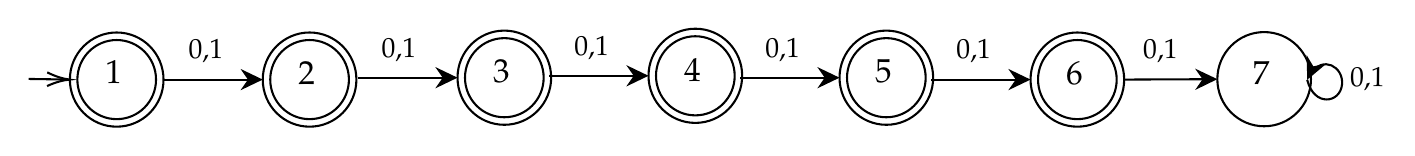
\begin{tikzpicture}[x=0.75pt,y=0.75pt,yscale=-1,xscale=1]
%uncomment if require: \path (0,78); %set diagram left start at 0, and has height of 78

%Shape: Ellipse [id:dp08566032050404582] 
\draw   (18.33,34.51) .. controls (18.33,21.98) and (28.43,11.82) .. (40.89,11.82) .. controls (53.35,11.82) and (63.45,21.98) .. (63.45,34.51) .. controls (63.45,47.04) and (53.35,57.2) .. (40.89,57.2) .. controls (28.43,57.2) and (18.33,47.04) .. (18.33,34.51) -- cycle ;
%Shape: Ellipse [id:dp5218579308315778] 
\draw   (111.26,34.51) .. controls (111.26,21.98) and (121.36,11.82) .. (133.82,11.82) .. controls (146.28,11.82) and (156.38,21.98) .. (156.38,34.51) .. controls (156.38,47.04) and (146.28,57.2) .. (133.82,57.2) .. controls (121.36,57.2) and (111.26,47.04) .. (111.26,34.51) -- cycle ;
%Straight Lines [id:da7079914981932862] 
\draw    (-1.5,34.2) -- (16.33,34.48) ;
\draw [shift={(18.33,34.51)}, rotate = 180.89] [color={rgb, 255:red, 0; green, 0; blue, 0 }  ][line width=0.75]    (10.93,-3.29) .. controls (6.95,-1.4) and (3.31,-0.3) .. (0,0) .. controls (3.31,0.3) and (6.95,1.4) .. (10.93,3.29)   ;
%Straight Lines [id:da5475256128923891] 
\draw    (63.45,34.51) -- (108.26,34.51) ;
\draw [shift={(111.26,34.51)}, rotate = 180] [fill={rgb, 255:red, 0; green, 0; blue, 0 }  ][line width=0.08]  [draw opacity=0] (10.72,-5.15) -- (0,0) -- (10.72,5.15) -- (7.12,0) -- cycle    ;
%Shape: Ellipse [id:dp7559245790181734] 
\draw   (205.1,33.6) .. controls (205.1,21.07) and (215.19,10.91) .. (227.65,10.91) .. controls (240.11,10.91) and (250.21,21.07) .. (250.21,33.6) .. controls (250.21,46.13) and (240.11,56.29) .. (227.65,56.29) .. controls (215.19,56.29) and (205.1,46.13) .. (205.1,33.6) -- cycle ;
%Straight Lines [id:da796961367907737] 
\draw    (157.28,33.6) -- (202.1,33.6) ;
\draw [shift={(205.1,33.6)}, rotate = 180] [fill={rgb, 255:red, 0; green, 0; blue, 0 }  ][line width=0.08]  [draw opacity=0] (10.72,-5.15) -- (0,0) -- (10.72,5.15) -- (7.12,0) -- cycle    ;
%Shape: Ellipse [id:dp18295492387511736] 
\draw   (297.12,32.69) .. controls (297.12,20.16) and (307.22,10) .. (319.68,10) .. controls (332.14,10) and (342.24,20.16) .. (342.24,32.69) .. controls (342.24,45.22) and (332.14,55.38) .. (319.68,55.38) .. controls (307.22,55.38) and (297.12,45.22) .. (297.12,32.69) -- cycle ;
%Straight Lines [id:da7147764359404827] 
\draw    (249.31,32.69) -- (294.12,32.69) ;
\draw [shift={(297.12,32.69)}, rotate = 180] [fill={rgb, 255:red, 0; green, 0; blue, 0 }  ][line width=0.08]  [draw opacity=0] (10.72,-5.15) -- (0,0) -- (10.72,5.15) -- (7.12,0) -- cycle    ;
%Shape: Ellipse [id:dp29554531887177005] 
\draw   (389.15,33.6) .. controls (389.15,21.07) and (399.25,10.91) .. (411.71,10.91) .. controls (424.16,10.91) and (434.26,21.07) .. (434.26,33.6) .. controls (434.26,46.13) and (424.16,56.29) .. (411.71,56.29) .. controls (399.25,56.29) and (389.15,46.13) .. (389.15,33.6) -- cycle ;
%Straight Lines [id:da9011541734821087] 
\draw    (341.33,33.6) -- (386.15,33.6) ;
\draw [shift={(389.15,33.6)}, rotate = 180] [fill={rgb, 255:red, 0; green, 0; blue, 0 }  ][line width=0.08]  [draw opacity=0] (10.72,-5.15) -- (0,0) -- (10.72,5.15) -- (7.12,0) -- cycle    ;
%Shape: Ellipse [id:dp6752522569320369] 
\draw   (481.18,34.51) .. controls (481.18,21.98) and (491.28,11.82) .. (503.74,11.82) .. controls (516.19,11.82) and (526.29,21.98) .. (526.29,34.51) .. controls (526.29,47.04) and (516.19,57.2) .. (503.74,57.2) .. controls (491.28,57.2) and (481.18,47.04) .. (481.18,34.51) -- cycle ;
%Straight Lines [id:da34251264906281764] 
\draw    (433.36,34.51) -- (478.18,34.51) ;
\draw [shift={(481.18,34.51)}, rotate = 180] [fill={rgb, 255:red, 0; green, 0; blue, 0 }  ][line width=0.08]  [draw opacity=0] (10.72,-5.15) -- (0,0) -- (10.72,5.15) -- (7.12,0) -- cycle    ;
%Shape: Ellipse [id:dp08029425228221476] 
\draw   (21.94,34.51) .. controls (21.94,23.98) and (30.43,15.45) .. (40.89,15.45) .. controls (51.35,15.45) and (59.84,23.98) .. (59.84,34.51) .. controls (59.84,45.04) and (51.35,53.57) .. (40.89,53.57) .. controls (30.43,53.57) and (21.94,45.04) .. (21.94,34.51) -- cycle ;
%Shape: Ellipse [id:dp5285178288062236] 
\draw   (114.87,34.51) .. controls (114.87,23.98) and (123.36,15.45) .. (133.82,15.45) .. controls (144.28,15.45) and (152.77,23.98) .. (152.77,34.51) .. controls (152.77,45.04) and (144.28,53.57) .. (133.82,53.57) .. controls (123.36,53.57) and (114.87,45.04) .. (114.87,34.51) -- cycle ;
%Shape: Ellipse [id:dp07915338546556261] 
\draw   (208.7,33.6) .. controls (208.7,23.07) and (217.19,14.54) .. (227.65,14.54) .. controls (238.12,14.54) and (246.6,23.07) .. (246.6,33.6) .. controls (246.6,44.13) and (238.12,52.66) .. (227.65,52.66) .. controls (217.19,52.66) and (208.7,44.13) .. (208.7,33.6) -- cycle ;
%Shape: Ellipse [id:dp7189508706911987] 
\draw   (300.73,32.69) .. controls (300.73,22.16) and (309.22,13.63) .. (319.68,13.63) .. controls (330.14,13.63) and (338.63,22.16) .. (338.63,32.69) .. controls (338.63,43.22) and (330.14,51.75) .. (319.68,51.75) .. controls (309.22,51.75) and (300.73,43.22) .. (300.73,32.69) -- cycle ;
%Shape: Ellipse [id:dp8065134465461772] 
\draw   (392.76,33.6) .. controls (392.76,23.07) and (401.24,14.54) .. (411.71,14.54) .. controls (422.17,14.54) and (430.65,23.07) .. (430.65,33.6) .. controls (430.65,44.13) and (422.17,52.66) .. (411.71,52.66) .. controls (401.24,52.66) and (392.76,44.13) .. (392.76,33.6) -- cycle ;
%Curve Lines [id:da2291470622863152] 
\draw    (614.47,34.61) .. controls (617.71,47.78) and (630.35,45.96) .. (631.25,36.88) .. controls (632.09,28.44) and (622,22.36) .. (615.79,32.13) ;
\draw [shift={(614.47,34.61)}, rotate = 294.34000000000003] [fill={rgb, 255:red, 0; green, 0; blue, 0 }  ][line width=0.08]  [draw opacity=0] (10.72,-5.15) -- (0,0) -- (10.72,5.15) -- (7.12,0) -- cycle    ;
%Shape: Ellipse [id:dp4650309065738025] 
\draw   (571.18,34.31) .. controls (571.18,21.78) and (581.28,11.62) .. (593.74,11.62) .. controls (606.19,11.62) and (616.29,21.78) .. (616.29,34.31) .. controls (616.29,46.84) and (606.19,57) .. (593.74,57) .. controls (581.28,57) and (571.18,46.84) .. (571.18,34.31) -- cycle ;
%Straight Lines [id:da20175781609916021] 
\draw    (526.29,34.51) -- (568.18,34.32) ;
\draw [shift={(571.18,34.31)}, rotate = 539.74] [fill={rgb, 255:red, 0; green, 0; blue, 0 }  ][line width=0.08]  [draw opacity=0] (10.72,-5.15) -- (0,0) -- (10.72,5.15) -- (7.12,0) -- cycle    ;
%Shape: Ellipse [id:dp3263947141536989] 
\draw   (484.79,34.51) .. controls (484.79,23.98) and (493.27,15.45) .. (503.74,15.45) .. controls (514.2,15.45) and (522.68,23.98) .. (522.68,34.51) .. controls (522.68,45.04) and (514.2,53.57) .. (503.74,53.57) .. controls (493.27,53.57) and (484.79,45.04) .. (484.79,34.51) -- cycle ;

% Text Node
\draw (33.99,23.55) node [anchor=north west][inner sep=0.75pt]  [font=\large] [align=left] {1};
% Text Node
\draw (126.92,24.46) node [anchor=north west][inner sep=0.75pt]  [font=\large] [align=left] {2};
% Text Node
\draw (74.05,13.75) node [anchor=north west][inner sep=0.75pt]   [align=left] {0,1};
% Text Node
\draw (220.75,23.55) node [anchor=north west][inner sep=0.75pt]  [font=\large] [align=left] {3};
% Text Node
\draw (166.98,12.85) node [anchor=north west][inner sep=0.75pt]   [align=left] {0,1};
% Text Node
\draw (312.78,22.65) node [anchor=north west][inner sep=0.75pt]  [font=\large] [align=left] {4};
% Text Node
\draw (259.91,11.94) node [anchor=north west][inner sep=0.75pt]   [align=left] {0,1};
% Text Node
\draw (404.81,23.55) node [anchor=north west][inner sep=0.75pt]  [font=\large] [align=left] {5};
% Text Node
\draw (351.94,12.85) node [anchor=north west][inner sep=0.75pt]   [align=left] {0,1};
% Text Node
\draw (496.83,24.46) node [anchor=north west][inner sep=0.75pt]  [font=\large] [align=left] {6};
% Text Node
\draw (443.97,13.75) node [anchor=north west][inner sep=0.75pt]   [align=left] {0,1};
% Text Node
\draw (633.71,26.97) node [anchor=north west][inner sep=0.75pt]  [rotate=-0.49] [align=left] {0,1};
% Text Node
\draw (586.83,24.26) node [anchor=north west][inner sep=0.75pt]  [font=\large] [align=left] {7};
% Text Node
\draw (533.97,13.55) node [anchor=north west][inner sep=0.75pt]   [align=left] {0,1};


\end{tikzpicture}

\item
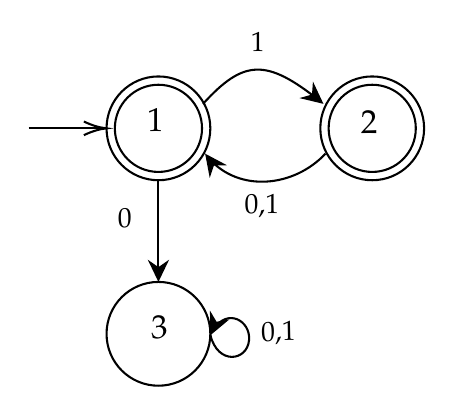
\begin{tikzpicture}[x=0.75pt,y=0.75pt,yscale=-1,xscale=1]
%uncomment if require: \path (0,238); %set diagram left start at 0, and has height of 238

%Shape: Circle [id:dp7531919938358536] 
\draw   (49,67) .. controls (49,53.19) and (60.19,42) .. (74,42) .. controls (87.81,42) and (99,53.19) .. (99,67) .. controls (99,80.81) and (87.81,92) .. (74,92) .. controls (60.19,92) and (49,80.81) .. (49,67) -- cycle ;
%Shape: Circle [id:dp26520015546954845] 
\draw   (156,67) .. controls (156,55.4) and (165.4,46) .. (177,46) .. controls (188.6,46) and (198,55.4) .. (198,67) .. controls (198,78.6) and (188.6,88) .. (177,88) .. controls (165.4,88) and (156,78.6) .. (156,67) -- cycle ;
%Shape: Circle [id:dp505689145184995] 
\draw   (152,67) .. controls (152,53.19) and (163.19,42) .. (177,42) .. controls (190.81,42) and (202,53.19) .. (202,67) .. controls (202,80.81) and (190.81,92) .. (177,92) .. controls (163.19,92) and (152,80.81) .. (152,67) -- cycle ;
%Straight Lines [id:da4329491393660516] 
\draw    (11.5,67) -- (47,67) ;
\draw [shift={(49,67)}, rotate = 180] [color={rgb, 255:red, 0; green, 0; blue, 0 }  ][line width=0.75]    (10.93,-3.29) .. controls (6.95,-1.4) and (3.31,-0.3) .. (0,0) .. controls (3.31,0.3) and (6.95,1.4) .. (10.93,3.29)   ;
%Shape: Circle [id:dp3882981606796625] 
\draw   (49,166) .. controls (49,152.19) and (60.19,141) .. (74,141) .. controls (87.81,141) and (99,152.19) .. (99,166) .. controls (99,179.81) and (87.81,191) .. (74,191) .. controls (60.19,191) and (49,179.81) .. (49,166) -- cycle ;
%Straight Lines [id:da33127173650729214] 
\draw    (74,92) -- (74,138) ;
\draw [shift={(74,141)}, rotate = 270] [fill={rgb, 255:red, 0; green, 0; blue, 0 }  ][line width=0.08]  [draw opacity=0] (10.72,-5.15) -- (0,0) -- (10.72,5.15) -- (7.12,0) -- cycle    ;
%Shape: Circle [id:dp1159308241860495] 
\draw   (53,67) .. controls (53,55.4) and (62.4,46) .. (74,46) .. controls (85.6,46) and (95,55.4) .. (95,67) .. controls (95,78.6) and (85.6,88) .. (74,88) .. controls (62.4,88) and (53,78.6) .. (53,67) -- cycle ;
%Curve Lines [id:da011299175297626585] 
\draw    (95.5,55.2) .. controls (115,33.75) and (125.94,33.21) .. (151.5,53.59) ;
\draw [shift={(153.5,55.2)}, rotate = 219.17000000000002] [fill={rgb, 255:red, 0; green, 0; blue, 0 }  ][line width=0.08]  [draw opacity=0] (10.72,-5.15) -- (0,0) -- (10.72,5.15) -- (7.12,0) -- cycle    ;
%Curve Lines [id:da6908760836736958] 
\draw    (154.5,79.2) .. controls (139.14,95.52) and (112.72,98.02) .. (98.25,81.38) ;
\draw [shift={(96.5,79.2)}, rotate = 413.62] [fill={rgb, 255:red, 0; green, 0; blue, 0 }  ][line width=0.08]  [draw opacity=0] (10.72,-5.15) -- (0,0) -- (10.72,5.15) -- (7.12,0) -- cycle    ;
%Curve Lines [id:da2023963932799706] 
\draw    (99.05,166.67) .. controls (102.65,181.17) and (116.65,179.17) .. (117.65,169.17) .. controls (118.58,159.82) and (107.28,153.09) .. (100.41,164.11) ;
\draw [shift={(99.05,166.67)}, rotate = 294.47] [fill={rgb, 255:red, 0; green, 0; blue, 0 }  ][line width=0.08]  [draw opacity=0] (10.72,-5.15) -- (0,0) -- (10.72,5.15) -- (7.12,0) -- cycle    ;

% Text Node
\draw (67,56) node [anchor=north west][inner sep=0.75pt]  [font=\large] [align=left] {1};
% Text Node
\draw (170,57) node [anchor=north west][inner sep=0.75pt]  [font=\large] [align=left] {2};
% Text Node
\draw (53,104) node [anchor=north west][inner sep=0.75pt]   [align=left] {0};
% Text Node
\draw (117,19) node [anchor=north west][inner sep=0.75pt]   [align=left] {1};
% Text Node
\draw (114,97) node [anchor=north west][inner sep=0.75pt]   [align=left] {0,1};
% Text Node
\draw (69,156) node [anchor=north west][inner sep=0.75pt]  [font=\large] [align=left] {3};
% Text Node
\draw (121.87,158.77) node [anchor=north west][inner sep=0.75pt]  [rotate=-358.81] [align=left] {0,1};


\end{tikzpicture}

\item
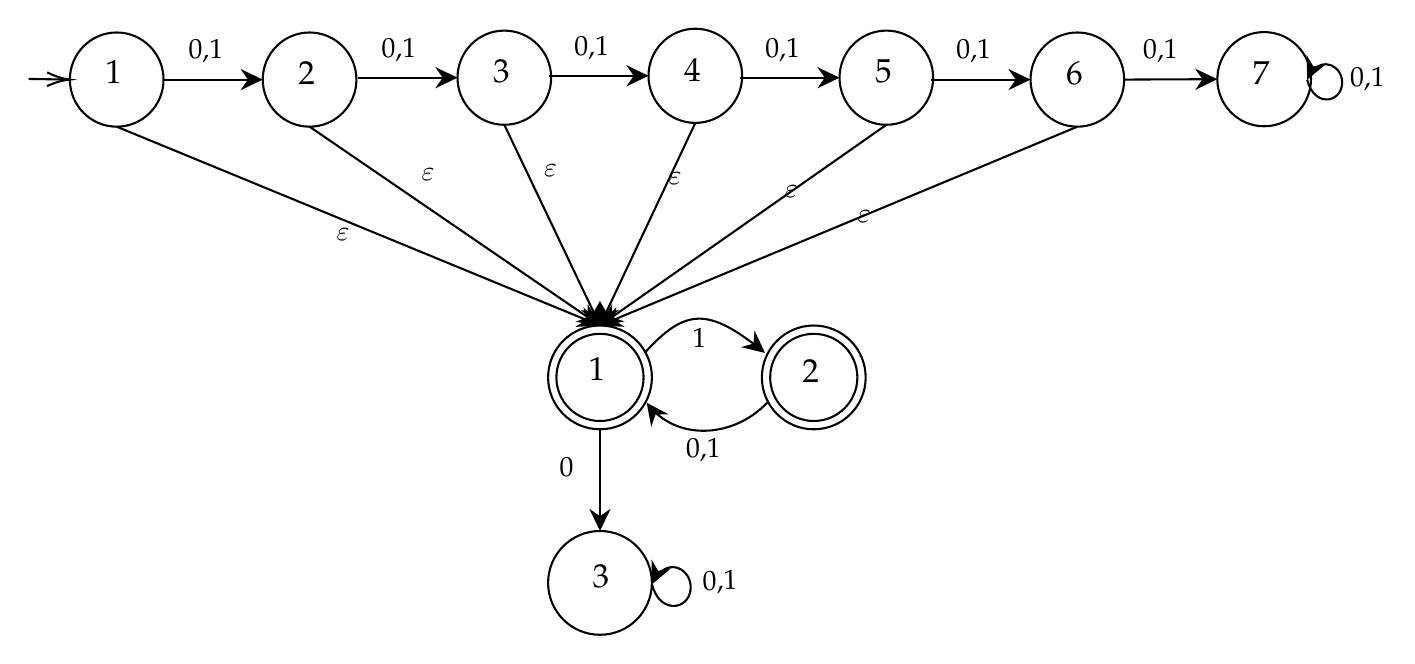
\begin{tikzpicture}[x=0.75pt,y=0.75pt,yscale=-1,xscale=1]
%uncomment if require: \path (0,326); %set diagram left start at 0, and has height of 326

%Shape: Circle [id:dp7575489959645265] 
\draw   (252,176) .. controls (252,162.19) and (263.19,151) .. (277,151) .. controls (290.81,151) and (302,162.19) .. (302,176) .. controls (302,189.81) and (290.81,201) .. (277,201) .. controls (263.19,201) and (252,189.81) .. (252,176) -- cycle ;
%Shape: Circle [id:dp7715044499176318] 
\draw   (359,176) .. controls (359,164.4) and (368.4,155) .. (380,155) .. controls (391.6,155) and (401,164.4) .. (401,176) .. controls (401,187.6) and (391.6,197) .. (380,197) .. controls (368.4,197) and (359,187.6) .. (359,176) -- cycle ;
%Shape: Circle [id:dp8111483150792473] 
\draw   (355,176) .. controls (355,162.19) and (366.19,151) .. (380,151) .. controls (393.81,151) and (405,162.19) .. (405,176) .. controls (405,189.81) and (393.81,201) .. (380,201) .. controls (366.19,201) and (355,189.81) .. (355,176) -- cycle ;
%Shape: Circle [id:dp5520799790740696] 
\draw   (252,275) .. controls (252,261.19) and (263.19,250) .. (277,250) .. controls (290.81,250) and (302,261.19) .. (302,275) .. controls (302,288.81) and (290.81,300) .. (277,300) .. controls (263.19,300) and (252,288.81) .. (252,275) -- cycle ;
%Straight Lines [id:da21398692774083905] 
\draw    (277,201) -- (277,247) ;
\draw [shift={(277,250)}, rotate = 270] [fill={rgb, 255:red, 0; green, 0; blue, 0 }  ][line width=0.08]  [draw opacity=0] (10.72,-5.15) -- (0,0) -- (10.72,5.15) -- (7.12,0) -- cycle    ;
%Shape: Circle [id:dp27253007811327623] 
\draw   (256,176) .. controls (256,164.4) and (265.4,155) .. (277,155) .. controls (288.6,155) and (298,164.4) .. (298,176) .. controls (298,187.6) and (288.6,197) .. (277,197) .. controls (265.4,197) and (256,187.6) .. (256,176) -- cycle ;
%Curve Lines [id:da25696601848881695] 
\draw    (298.5,164.2) .. controls (318,142.75) and (328.94,142.21) .. (354.5,162.59) ;
\draw [shift={(356.5,164.2)}, rotate = 219.17000000000002] [fill={rgb, 255:red, 0; green, 0; blue, 0 }  ][line width=0.08]  [draw opacity=0] (10.72,-5.15) -- (0,0) -- (10.72,5.15) -- (7.12,0) -- cycle    ;
%Curve Lines [id:da8255204965122127] 
\draw    (357.5,188.2) .. controls (342.14,204.52) and (315.72,207.02) .. (301.25,190.38) ;
\draw [shift={(299.5,188.2)}, rotate = 413.62] [fill={rgb, 255:red, 0; green, 0; blue, 0 }  ][line width=0.08]  [draw opacity=0] (10.72,-5.15) -- (0,0) -- (10.72,5.15) -- (7.12,0) -- cycle    ;
%Curve Lines [id:da8957959715464072] 
\draw    (302.05,275.67) .. controls (305.65,290.17) and (319.65,288.17) .. (320.65,278.17) .. controls (321.58,268.82) and (310.28,262.09) .. (303.41,273.11) ;
\draw [shift={(302.05,275.67)}, rotate = 294.47] [fill={rgb, 255:red, 0; green, 0; blue, 0 }  ][line width=0.08]  [draw opacity=0] (10.72,-5.15) -- (0,0) -- (10.72,5.15) -- (7.12,0) -- cycle    ;
%Shape: Ellipse [id:dp8374575191651707] 
\draw   (21.59,32.51) .. controls (21.59,19.98) and (31.69,9.82) .. (44.15,9.82) .. controls (56.61,9.82) and (66.71,19.98) .. (66.71,32.51) .. controls (66.71,45.04) and (56.61,55.2) .. (44.15,55.2) .. controls (31.69,55.2) and (21.59,45.04) .. (21.59,32.51) -- cycle ;
%Shape: Ellipse [id:dp9880306602753175] 
\draw   (114.52,32.51) .. controls (114.52,19.98) and (124.62,9.82) .. (137.08,9.82) .. controls (149.54,9.82) and (159.64,19.98) .. (159.64,32.51) .. controls (159.64,45.04) and (149.54,55.2) .. (137.08,55.2) .. controls (124.62,55.2) and (114.52,45.04) .. (114.52,32.51) -- cycle ;
%Straight Lines [id:da2591568719726767] 
\draw    (1.76,32.2) -- (19.59,32.48) ;
\draw [shift={(21.59,32.51)}, rotate = 180.89] [color={rgb, 255:red, 0; green, 0; blue, 0 }  ][line width=0.75]    (10.93,-3.29) .. controls (6.95,-1.4) and (3.31,-0.3) .. (0,0) .. controls (3.31,0.3) and (6.95,1.4) .. (10.93,3.29)   ;
%Straight Lines [id:da39778457367154285] 
\draw    (66.71,32.51) -- (111.52,32.51) ;
\draw [shift={(114.52,32.51)}, rotate = 180] [fill={rgb, 255:red, 0; green, 0; blue, 0 }  ][line width=0.08]  [draw opacity=0] (10.72,-5.15) -- (0,0) -- (10.72,5.15) -- (7.12,0) -- cycle    ;
%Shape: Ellipse [id:dp1658109491684927] 
\draw   (208.36,31.6) .. controls (208.36,19.07) and (218.45,8.91) .. (230.91,8.91) .. controls (243.37,8.91) and (253.47,19.07) .. (253.47,31.6) .. controls (253.47,44.13) and (243.37,54.29) .. (230.91,54.29) .. controls (218.45,54.29) and (208.36,44.13) .. (208.36,31.6) -- cycle ;
%Straight Lines [id:da22544115319219737] 
\draw    (160.54,31.6) -- (205.36,31.6) ;
\draw [shift={(208.36,31.6)}, rotate = 180] [fill={rgb, 255:red, 0; green, 0; blue, 0 }  ][line width=0.08]  [draw opacity=0] (10.72,-5.15) -- (0,0) -- (10.72,5.15) -- (7.12,0) -- cycle    ;
%Shape: Ellipse [id:dp8536438687232997] 
\draw   (300.38,30.69) .. controls (300.38,18.16) and (310.48,8) .. (322.94,8) .. controls (335.4,8) and (345.5,18.16) .. (345.5,30.69) .. controls (345.5,43.22) and (335.4,53.38) .. (322.94,53.38) .. controls (310.48,53.38) and (300.38,43.22) .. (300.38,30.69) -- cycle ;
%Straight Lines [id:da07567321526907156] 
\draw    (252.57,30.69) -- (297.38,30.69) ;
\draw [shift={(300.38,30.69)}, rotate = 180] [fill={rgb, 255:red, 0; green, 0; blue, 0 }  ][line width=0.08]  [draw opacity=0] (10.72,-5.15) -- (0,0) -- (10.72,5.15) -- (7.12,0) -- cycle    ;
%Shape: Ellipse [id:dp8854809009821081] 
\draw   (392.41,31.6) .. controls (392.41,19.07) and (402.51,8.91) .. (414.97,8.91) .. controls (427.42,8.91) and (437.52,19.07) .. (437.52,31.6) .. controls (437.52,44.13) and (427.42,54.29) .. (414.97,54.29) .. controls (402.51,54.29) and (392.41,44.13) .. (392.41,31.6) -- cycle ;
%Straight Lines [id:da49413294324533585] 
\draw    (344.59,31.6) -- (389.41,31.6) ;
\draw [shift={(392.41,31.6)}, rotate = 180] [fill={rgb, 255:red, 0; green, 0; blue, 0 }  ][line width=0.08]  [draw opacity=0] (10.72,-5.15) -- (0,0) -- (10.72,5.15) -- (7.12,0) -- cycle    ;
%Shape: Ellipse [id:dp43798386156848945] 
\draw   (484.44,32.51) .. controls (484.44,19.98) and (494.54,9.82) .. (506.99,9.82) .. controls (519.45,9.82) and (529.55,19.98) .. (529.55,32.51) .. controls (529.55,45.04) and (519.45,55.2) .. (506.99,55.2) .. controls (494.54,55.2) and (484.44,45.04) .. (484.44,32.51) -- cycle ;
%Straight Lines [id:da7409259918160738] 
\draw    (436.62,32.51) -- (481.44,32.51) ;
\draw [shift={(484.44,32.51)}, rotate = 180] [fill={rgb, 255:red, 0; green, 0; blue, 0 }  ][line width=0.08]  [draw opacity=0] (10.72,-5.15) -- (0,0) -- (10.72,5.15) -- (7.12,0) -- cycle    ;
%Curve Lines [id:da6456937261417459] 
\draw    (617.73,32.61) .. controls (620.97,45.78) and (633.6,43.96) .. (634.51,34.88) .. controls (635.35,26.44) and (625.26,20.36) .. (619.05,30.13) ;
\draw [shift={(617.73,32.61)}, rotate = 294.34000000000003] [fill={rgb, 255:red, 0; green, 0; blue, 0 }  ][line width=0.08]  [draw opacity=0] (10.72,-5.15) -- (0,0) -- (10.72,5.15) -- (7.12,0) -- cycle    ;
%Shape: Ellipse [id:dp22759689017891582] 
\draw   (574.44,32.31) .. controls (574.44,19.78) and (584.54,9.62) .. (596.99,9.62) .. controls (609.45,9.62) and (619.55,19.78) .. (619.55,32.31) .. controls (619.55,44.84) and (609.45,55) .. (596.99,55) .. controls (584.54,55) and (574.44,44.84) .. (574.44,32.31) -- cycle ;
%Straight Lines [id:da22037335084640075] 
\draw    (529.55,32.51) -- (571.44,32.32) ;
\draw [shift={(574.44,32.31)}, rotate = 539.74] [fill={rgb, 255:red, 0; green, 0; blue, 0 }  ][line width=0.08]  [draw opacity=0] (10.72,-5.15) -- (0,0) -- (10.72,5.15) -- (7.12,0) -- cycle    ;
%Straight Lines [id:da8020945812492561] 
\draw    (44.15,55.2) -- (274.23,149.86) ;
\draw [shift={(277,151)}, rotate = 202.36] [fill={rgb, 255:red, 0; green, 0; blue, 0 }  ][line width=0.08]  [draw opacity=0] (10.72,-5.15) -- (0,0) -- (10.72,5.15) -- (7.12,0) -- cycle    ;
%Straight Lines [id:da8181295657217935] 
\draw    (137.08,55.2) -- (274.52,149.31) ;
\draw [shift={(277,151)}, rotate = 214.4] [fill={rgb, 255:red, 0; green, 0; blue, 0 }  ][line width=0.08]  [draw opacity=0] (10.72,-5.15) -- (0,0) -- (10.72,5.15) -- (7.12,0) -- cycle    ;
%Straight Lines [id:da887648526178904] 
\draw    (230.91,54.29) -- (275.71,148.29) ;
\draw [shift={(277,151)}, rotate = 244.51999999999998] [fill={rgb, 255:red, 0; green, 0; blue, 0 }  ][line width=0.08]  [draw opacity=0] (10.72,-5.15) -- (0,0) -- (10.72,5.15) -- (7.12,0) -- cycle    ;
%Straight Lines [id:da09746548030068647] 
\draw    (322.94,53.38) -- (278.28,148.29) ;
\draw [shift={(277,151)}, rotate = 295.2] [fill={rgb, 255:red, 0; green, 0; blue, 0 }  ][line width=0.08]  [draw opacity=0] (10.72,-5.15) -- (0,0) -- (10.72,5.15) -- (7.12,0) -- cycle    ;
%Straight Lines [id:da13255524357789183] 
\draw    (414.97,54.29) -- (279.46,149.28) ;
\draw [shift={(277,151)}, rotate = 324.97] [fill={rgb, 255:red, 0; green, 0; blue, 0 }  ][line width=0.08]  [draw opacity=0] (10.72,-5.15) -- (0,0) -- (10.72,5.15) -- (7.12,0) -- cycle    ;
%Straight Lines [id:da17729220026438908] 
\draw    (506.99,55.2) -- (279.77,149.85) ;
\draw [shift={(277,151)}, rotate = 337.39] [fill={rgb, 255:red, 0; green, 0; blue, 0 }  ][line width=0.08]  [draw opacity=0] (10.72,-5.15) -- (0,0) -- (10.72,5.15) -- (7.12,0) -- cycle    ;

% Text Node
\draw (270,165) node [anchor=north west][inner sep=0.75pt]  [font=\large] [align=left] {1};
% Text Node
\draw (373,166) node [anchor=north west][inner sep=0.75pt]  [font=\large] [align=left] {2};
% Text Node
\draw (256,213) node [anchor=north west][inner sep=0.75pt]   [align=left] {0};
% Text Node
\draw (320,151) node [anchor=north west][inner sep=0.75pt]   [align=left] {1};
% Text Node
\draw (317,204) node [anchor=north west][inner sep=0.75pt]   [align=left] {0,1};
% Text Node
\draw (272,265) node [anchor=north west][inner sep=0.75pt]  [font=\large] [align=left] {3};
% Text Node
\draw (324.87,267.77) node [anchor=north west][inner sep=0.75pt]  [rotate=-358.81] [align=left] {0,1};
% Text Node
\draw (37.25,21.55) node [anchor=north west][inner sep=0.75pt]  [font=\large] [align=left] {1};
% Text Node
\draw (130.18,22.46) node [anchor=north west][inner sep=0.75pt]  [font=\large] [align=left] {2};
% Text Node
\draw (77.31,11.75) node [anchor=north west][inner sep=0.75pt]   [align=left] {0,1};
% Text Node
\draw (224.01,21.55) node [anchor=north west][inner sep=0.75pt]  [font=\large] [align=left] {3};
% Text Node
\draw (170.24,10.85) node [anchor=north west][inner sep=0.75pt]   [align=left] {0,1};
% Text Node
\draw (316.04,20.65) node [anchor=north west][inner sep=0.75pt]  [font=\large] [align=left] {4};
% Text Node
\draw (263.17,9.94) node [anchor=north west][inner sep=0.75pt]   [align=left] {0,1};
% Text Node
\draw (408.06,21.55) node [anchor=north west][inner sep=0.75pt]  [font=\large] [align=left] {5};
% Text Node
\draw (355.2,10.85) node [anchor=north west][inner sep=0.75pt]   [align=left] {0,1};
% Text Node
\draw (500.09,22.46) node [anchor=north west][inner sep=0.75pt]  [font=\large] [align=left] {6};
% Text Node
\draw (447.23,11.75) node [anchor=north west][inner sep=0.75pt]   [align=left] {0,1};
% Text Node
\draw (636.97,24.97) node [anchor=north west][inner sep=0.75pt]  [rotate=-0.49] [align=left] {0,1};
% Text Node
\draw (590.09,22.26) node [anchor=north west][inner sep=0.75pt]  [font=\large] [align=left] {7};
% Text Node
\draw (537.23,11.55) node [anchor=north west][inner sep=0.75pt]   [align=left] {0,1};
% Text Node
\draw (148.66,103.02) node [anchor=north west][inner sep=0.75pt]  [rotate=-0.49] [align=left] {$\displaystyle \varepsilon $};
% Text Node
\draw (189.66,74.02) node [anchor=north west][inner sep=0.75pt]  [rotate=-0.49] [align=left] {$\displaystyle \varepsilon $};
% Text Node
\draw (248.66,72.02) node [anchor=north west][inner sep=0.75pt]  [rotate=-0.49] [align=left] {$\displaystyle \varepsilon $};
% Text Node
\draw (308.66,76.02) node [anchor=north west][inner sep=0.75pt]  [rotate=-0.49] [align=left] {$\displaystyle \varepsilon $};
% Text Node
\draw (364.66,82.02) node [anchor=north west][inner sep=0.75pt]  [rotate=-0.49] [align=left] {$\displaystyle \varepsilon $};
% Text Node
\draw (399.66,94.02) node [anchor=north west][inner sep=0.75pt]  [rotate=-0.49] [align=left] {$\displaystyle \varepsilon $};


\end{tikzpicture}


\end{enumerate}

\newpage

\begin{prob}\end{prob}

\begin{enumerate}[label=(\alph*)]

\item
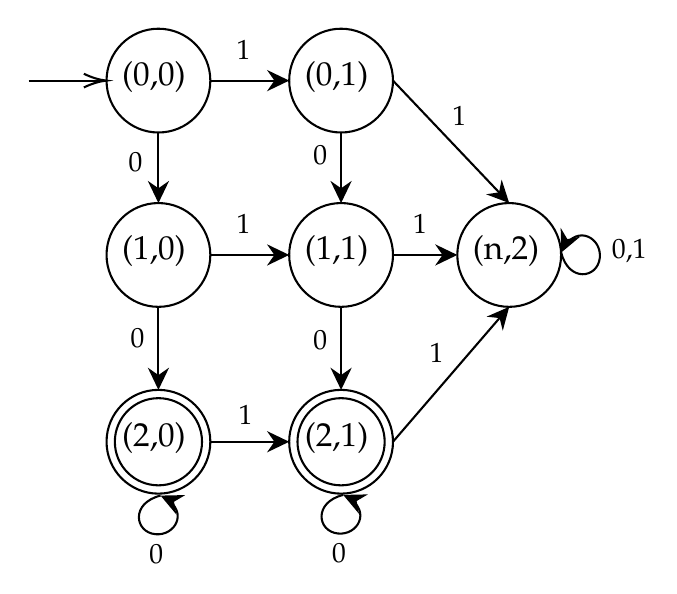
\begin{tikzpicture}[x=0.75pt,y=0.75pt,yscale=-1,xscale=1]
%uncomment if require: \path (0,290); %set diagram left start at 0, and has height of 290

%Shape: Circle [id:dp11055406943256108] 
\draw   (57,39) .. controls (57,25.19) and (68.19,14) .. (82,14) .. controls (95.81,14) and (107,25.19) .. (107,39) .. controls (107,52.81) and (95.81,64) .. (82,64) .. controls (68.19,64) and (57,52.81) .. (57,39) -- cycle ;
%Straight Lines [id:da4980267526699602] 
\draw    (19.5,39) -- (55,39) ;
\draw [shift={(57,39)}, rotate = 180] [color={rgb, 255:red, 0; green, 0; blue, 0 }  ][line width=0.75]    (10.93,-3.29) .. controls (6.95,-1.4) and (3.31,-0.3) .. (0,0) .. controls (3.31,0.3) and (6.95,1.4) .. (10.93,3.29)   ;
%Shape: Circle [id:dp24089692735961865] 
\draw   (145,39) .. controls (145,25.19) and (156.19,14) .. (170,14) .. controls (183.81,14) and (195,25.19) .. (195,39) .. controls (195,52.81) and (183.81,64) .. (170,64) .. controls (156.19,64) and (145,52.81) .. (145,39) -- cycle ;
%Straight Lines [id:da24205454931303994] 
\draw    (107,39) -- (142,39) ;
\draw [shift={(145,39)}, rotate = 180] [fill={rgb, 255:red, 0; green, 0; blue, 0 }  ][line width=0.08]  [draw opacity=0] (10.72,-5.15) -- (0,0) -- (10.72,5.15) -- (7.12,0) -- cycle    ;
%Shape: Circle [id:dp3511575575466459] 
\draw   (57,123) .. controls (57,109.19) and (68.19,98) .. (82,98) .. controls (95.81,98) and (107,109.19) .. (107,123) .. controls (107,136.81) and (95.81,148) .. (82,148) .. controls (68.19,148) and (57,136.81) .. (57,123) -- cycle ;
%Shape: Circle [id:dp5743845564234975] 
\draw   (145,123) .. controls (145,109.19) and (156.19,98) .. (170,98) .. controls (183.81,98) and (195,109.19) .. (195,123) .. controls (195,136.81) and (183.81,148) .. (170,148) .. controls (156.19,148) and (145,136.81) .. (145,123) -- cycle ;
%Shape: Circle [id:dp024154206083003338] 
\draw   (57,213) .. controls (57,199.19) and (68.19,188) .. (82,188) .. controls (95.81,188) and (107,199.19) .. (107,213) .. controls (107,226.81) and (95.81,238) .. (82,238) .. controls (68.19,238) and (57,226.81) .. (57,213) -- cycle ;
%Shape: Circle [id:dp7020123996235517] 
\draw   (145,213) .. controls (145,199.19) and (156.19,188) .. (170,188) .. controls (183.81,188) and (195,199.19) .. (195,213) .. controls (195,226.81) and (183.81,238) .. (170,238) .. controls (156.19,238) and (145,226.81) .. (145,213) -- cycle ;
%Straight Lines [id:da2758305610550862] 
\draw    (82,64) -- (82,95) ;
\draw [shift={(82,98)}, rotate = 270] [fill={rgb, 255:red, 0; green, 0; blue, 0 }  ][line width=0.08]  [draw opacity=0] (10.72,-5.15) -- (0,0) -- (10.72,5.15) -- (7.12,0) -- cycle    ;
%Straight Lines [id:da02079485432578987] 
\draw    (170,64) -- (170,95) ;
\draw [shift={(170,98)}, rotate = 270] [fill={rgb, 255:red, 0; green, 0; blue, 0 }  ][line width=0.08]  [draw opacity=0] (10.72,-5.15) -- (0,0) -- (10.72,5.15) -- (7.12,0) -- cycle    ;
%Straight Lines [id:da11542890640330628] 
\draw    (82,148) -- (82,185) ;
\draw [shift={(82,188)}, rotate = 270] [fill={rgb, 255:red, 0; green, 0; blue, 0 }  ][line width=0.08]  [draw opacity=0] (10.72,-5.15) -- (0,0) -- (10.72,5.15) -- (7.12,0) -- cycle    ;
%Straight Lines [id:da7850136668208201] 
\draw    (107,123) -- (142,123) ;
\draw [shift={(145,123)}, rotate = 180] [fill={rgb, 255:red, 0; green, 0; blue, 0 }  ][line width=0.08]  [draw opacity=0] (10.72,-5.15) -- (0,0) -- (10.72,5.15) -- (7.12,0) -- cycle    ;
%Straight Lines [id:da5315232670271082] 
\draw    (107,213) -- (142,213) ;
\draw [shift={(145,213)}, rotate = 180] [fill={rgb, 255:red, 0; green, 0; blue, 0 }  ][line width=0.08]  [draw opacity=0] (10.72,-5.15) -- (0,0) -- (10.72,5.15) -- (7.12,0) -- cycle    ;
%Straight Lines [id:da8548915881040959] 
\draw    (170,148) -- (170,185) ;
\draw [shift={(170,188)}, rotate = 270] [fill={rgb, 255:red, 0; green, 0; blue, 0 }  ][line width=0.08]  [draw opacity=0] (10.72,-5.15) -- (0,0) -- (10.72,5.15) -- (7.12,0) -- cycle    ;
%Shape: Circle [id:dp8553813621284929] 
\draw   (226,123) .. controls (226,109.19) and (237.19,98) .. (251,98) .. controls (264.81,98) and (276,109.19) .. (276,123) .. controls (276,136.81) and (264.81,148) .. (251,148) .. controls (237.19,148) and (226,136.81) .. (226,123) -- cycle ;
%Straight Lines [id:da6918381530241942] 
\draw    (195,123) -- (223,123) ;
\draw [shift={(226,123)}, rotate = 180] [fill={rgb, 255:red, 0; green, 0; blue, 0 }  ][line width=0.08]  [draw opacity=0] (10.72,-5.15) -- (0,0) -- (10.72,5.15) -- (7.12,0) -- cycle    ;
%Straight Lines [id:da930857863717431] 
\draw    (195,39) -- (248.93,95.82) ;
\draw [shift={(251,98)}, rotate = 226.49] [fill={rgb, 255:red, 0; green, 0; blue, 0 }  ][line width=0.08]  [draw opacity=0] (10.72,-5.15) -- (0,0) -- (10.72,5.15) -- (7.12,0) -- cycle    ;
%Straight Lines [id:da30433529113979163] 
\draw    (195,213) -- (249.04,150.27) ;
\draw [shift={(251,148)}, rotate = 490.75] [fill={rgb, 255:red, 0; green, 0; blue, 0 }  ][line width=0.08]  [draw opacity=0] (10.72,-5.15) -- (0,0) -- (10.72,5.15) -- (7.12,0) -- cycle    ;
%Shape: Circle [id:dp31653068713080224] 
\draw   (61,213) .. controls (61,201.4) and (70.4,192) .. (82,192) .. controls (93.6,192) and (103,201.4) .. (103,213) .. controls (103,224.6) and (93.6,234) .. (82,234) .. controls (70.4,234) and (61,224.6) .. (61,213) -- cycle ;
%Shape: Circle [id:dp6441790319259328] 
\draw   (149,213) .. controls (149,201.4) and (158.4,192) .. (170,192) .. controls (181.6,192) and (191,201.4) .. (191,213) .. controls (191,224.6) and (181.6,234) .. (170,234) .. controls (158.4,234) and (149,224.6) .. (149,213) -- cycle ;
%Curve Lines [id:da4726576813684775] 
\draw    (276.05,121.85) .. controls (279.65,136.35) and (293.65,134.35) .. (294.65,124.35) .. controls (295.58,115) and (284.28,108.27) .. (277.41,119.29) ;
\draw [shift={(276.05,121.85)}, rotate = 294.47] [fill={rgb, 255:red, 0; green, 0; blue, 0 }  ][line width=0.08]  [draw opacity=0] (10.72,-5.15) -- (0,0) -- (10.72,5.15) -- (7.12,0) -- cycle    ;
%Curve Lines [id:da24842945462640587] 
\draw    (171.02,238.61) .. controls (156.52,242.21) and (158.52,256.21) .. (168.52,257.21) .. controls (177.87,258.15) and (184.59,246.84) .. (173.58,239.97) ;
\draw [shift={(171.02,238.61)}, rotate = 384.47] [fill={rgb, 255:red, 0; green, 0; blue, 0 }  ][line width=0.08]  [draw opacity=0] (10.72,-5.15) -- (0,0) -- (10.72,5.15) -- (7.12,0) -- cycle    ;
%Curve Lines [id:da10803550155441477] 
\draw    (83.02,238.94) .. controls (68.52,242.54) and (70.52,256.54) .. (80.52,257.54) .. controls (89.87,258.48) and (96.59,247.17) .. (85.58,240.3) ;
\draw [shift={(83.02,238.94)}, rotate = 384.47] [fill={rgb, 255:red, 0; green, 0; blue, 0 }  ][line width=0.08]  [draw opacity=0] (10.72,-5.15) -- (0,0) -- (10.72,5.15) -- (7.12,0) -- cycle    ;

% Text Node
\draw (63,28) node [anchor=north west][inner sep=0.75pt]  [font=\large] [align=left] {(0,0)};
% Text Node
\draw (151,28) node [anchor=north west][inner sep=0.75pt]  [font=\large] [align=left] {(0,1)};
% Text Node
\draw (63,112) node [anchor=north west][inner sep=0.75pt]  [font=\large] [align=left] {(1,0)};
% Text Node
\draw (151,112) node [anchor=north west][inner sep=0.75pt]  [font=\large] [align=left] {(1,1)};
% Text Node
\draw (63,202) node [anchor=north west][inner sep=0.75pt]  [font=\large] [align=left] {(2,0)};
% Text Node
\draw (151,202) node [anchor=north west][inner sep=0.75pt]  [font=\large] [align=left] {(2,1)};
% Text Node
\draw (232,112) node [anchor=north west][inner sep=0.75pt]  [font=\large] [align=left] {(n,2)};
% Text Node
\draw (298.87,113.96) node [anchor=north west][inner sep=0.75pt]  [rotate=-358.81] [align=left] {0,1};
% Text Node
\draw (164.11,260.66) node [anchor=north west][inner sep=0.75pt]  [rotate=-359.73] [align=left] {0};
% Text Node
\draw (76.11,260.99) node [anchor=north west][inner sep=0.75pt]  [rotate=-359.73] [align=left] {0};
% Text Node
\draw (67.11,156.99) node [anchor=north west][inner sep=0.75pt]  [rotate=-359.73] [align=left] {0};
% Text Node
\draw (66.11,71.99) node [anchor=north west][inner sep=0.75pt]  [rotate=-359.73] [align=left] {0};
% Text Node
\draw (155.11,157.99) node [anchor=north west][inner sep=0.75pt]  [rotate=-359.73] [align=left] {0};
% Text Node
\draw (155.11,68.99) node [anchor=north west][inner sep=0.75pt]  [rotate=-359.73] [align=left] {0};
% Text Node
\draw (118.11,17.99) node [anchor=north west][inner sep=0.75pt]  [rotate=-359.73] [align=left] {1};
% Text Node
\draw (118.11,101.99) node [anchor=north west][inner sep=0.75pt]  [rotate=-359.73] [align=left] {1};
% Text Node
\draw (119.11,193.99) node [anchor=north west][inner sep=0.75pt]  [rotate=-359.73] [align=left] {1};
% Text Node
\draw (222.11,49.99) node [anchor=north west][inner sep=0.75pt]  [rotate=-359.73] [align=left] {1};
% Text Node
\draw (203.11,101.99) node [anchor=north west][inner sep=0.75pt]  [rotate=-359.73] [align=left] {1};
% Text Node
\draw (211.11,163.99) node [anchor=north west][inner sep=0.75pt]  [rotate=-359.73] [align=left] {1};


\end{tikzpicture}

where the states are roughly organized as an ordered pair $(q_1, q_2)$, where $q_1$ represents the number of zeroes,
and $q_2$ represents the number of ones. $(n, 2)$ is a trap state where we've exceeded the maximum number of ones (1).

\item
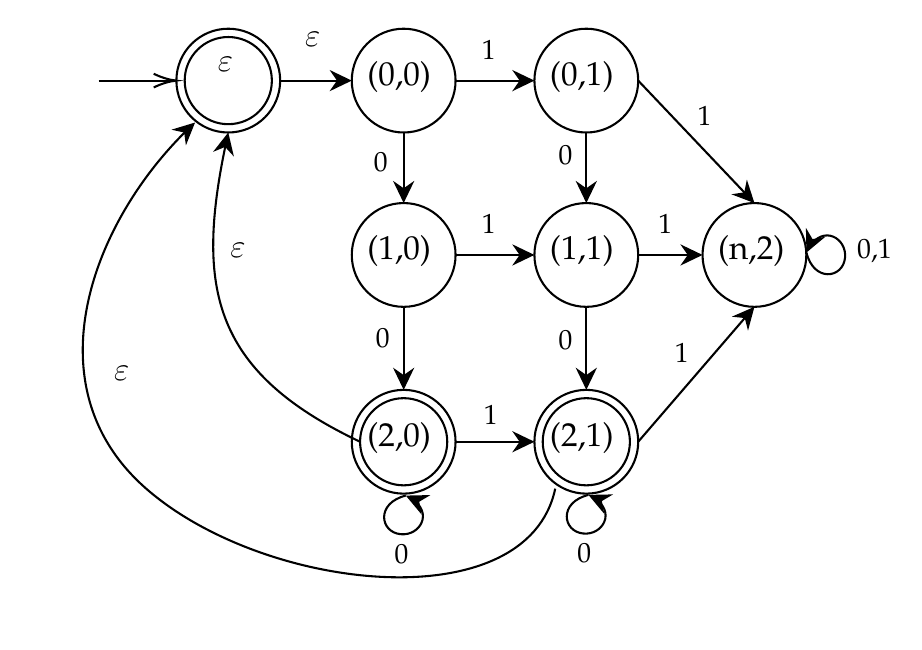
\begin{tikzpicture}[x=0.75pt,y=0.75pt,yscale=-1,xscale=1]
%uncomment if require: \path (0,300); %set diagram left start at 0, and has height of 300

%Shape: Circle [id:dp1640362802023707] 
\draw   (157,41) .. controls (157,27.19) and (168.19,16) .. (182,16) .. controls (195.81,16) and (207,27.19) .. (207,41) .. controls (207,54.81) and (195.81,66) .. (182,66) .. controls (168.19,66) and (157,54.81) .. (157,41) -- cycle ;
%Straight Lines [id:da740198435192776] 
\draw    (35,41) -- (59,41) -- (70.5,41) ;
\draw [shift={(72.5,41)}, rotate = 180] [color={rgb, 255:red, 0; green, 0; blue, 0 }  ][line width=0.75]    (10.93,-3.29) .. controls (6.95,-1.4) and (3.31,-0.3) .. (0,0) .. controls (3.31,0.3) and (6.95,1.4) .. (10.93,3.29)   ;
%Shape: Circle [id:dp5904822366619515] 
\draw   (245,41) .. controls (245,27.19) and (256.19,16) .. (270,16) .. controls (283.81,16) and (295,27.19) .. (295,41) .. controls (295,54.81) and (283.81,66) .. (270,66) .. controls (256.19,66) and (245,54.81) .. (245,41) -- cycle ;
%Straight Lines [id:da36146789363784304] 
\draw    (207,41) -- (242,41) ;
\draw [shift={(245,41)}, rotate = 180] [fill={rgb, 255:red, 0; green, 0; blue, 0 }  ][line width=0.08]  [draw opacity=0] (10.72,-5.15) -- (0,0) -- (10.72,5.15) -- (7.12,0) -- cycle    ;
%Shape: Circle [id:dp6577418315015529] 
\draw   (157,125) .. controls (157,111.19) and (168.19,100) .. (182,100) .. controls (195.81,100) and (207,111.19) .. (207,125) .. controls (207,138.81) and (195.81,150) .. (182,150) .. controls (168.19,150) and (157,138.81) .. (157,125) -- cycle ;
%Shape: Circle [id:dp5452901718394154] 
\draw   (245,125) .. controls (245,111.19) and (256.19,100) .. (270,100) .. controls (283.81,100) and (295,111.19) .. (295,125) .. controls (295,138.81) and (283.81,150) .. (270,150) .. controls (256.19,150) and (245,138.81) .. (245,125) -- cycle ;
%Shape: Circle [id:dp6256398576371742] 
\draw   (157,215) .. controls (157,201.19) and (168.19,190) .. (182,190) .. controls (195.81,190) and (207,201.19) .. (207,215) .. controls (207,228.81) and (195.81,240) .. (182,240) .. controls (168.19,240) and (157,228.81) .. (157,215) -- cycle ;
%Shape: Circle [id:dp8704612205753213] 
\draw   (245,215) .. controls (245,201.19) and (256.19,190) .. (270,190) .. controls (283.81,190) and (295,201.19) .. (295,215) .. controls (295,228.81) and (283.81,240) .. (270,240) .. controls (256.19,240) and (245,228.81) .. (245,215) -- cycle ;
%Straight Lines [id:da24194196009320823] 
\draw    (182,66) -- (182,97) ;
\draw [shift={(182,100)}, rotate = 270] [fill={rgb, 255:red, 0; green, 0; blue, 0 }  ][line width=0.08]  [draw opacity=0] (10.72,-5.15) -- (0,0) -- (10.72,5.15) -- (7.12,0) -- cycle    ;
%Straight Lines [id:da5913420265335536] 
\draw    (270,66) -- (270,97) ;
\draw [shift={(270,100)}, rotate = 270] [fill={rgb, 255:red, 0; green, 0; blue, 0 }  ][line width=0.08]  [draw opacity=0] (10.72,-5.15) -- (0,0) -- (10.72,5.15) -- (7.12,0) -- cycle    ;
%Straight Lines [id:da03749235117826033] 
\draw    (182,150) -- (182,187) ;
\draw [shift={(182,190)}, rotate = 270] [fill={rgb, 255:red, 0; green, 0; blue, 0 }  ][line width=0.08]  [draw opacity=0] (10.72,-5.15) -- (0,0) -- (10.72,5.15) -- (7.12,0) -- cycle    ;
%Straight Lines [id:da3962559679246249] 
\draw    (207,125) -- (242,125) ;
\draw [shift={(245,125)}, rotate = 180] [fill={rgb, 255:red, 0; green, 0; blue, 0 }  ][line width=0.08]  [draw opacity=0] (10.72,-5.15) -- (0,0) -- (10.72,5.15) -- (7.12,0) -- cycle    ;
%Straight Lines [id:da27301468376460414] 
\draw    (207,215) -- (242,215) ;
\draw [shift={(245,215)}, rotate = 180] [fill={rgb, 255:red, 0; green, 0; blue, 0 }  ][line width=0.08]  [draw opacity=0] (10.72,-5.15) -- (0,0) -- (10.72,5.15) -- (7.12,0) -- cycle    ;
%Straight Lines [id:da4599252143688468] 
\draw    (270,150) -- (270,187) ;
\draw [shift={(270,190)}, rotate = 270] [fill={rgb, 255:red, 0; green, 0; blue, 0 }  ][line width=0.08]  [draw opacity=0] (10.72,-5.15) -- (0,0) -- (10.72,5.15) -- (7.12,0) -- cycle    ;
%Shape: Circle [id:dp03135552647120732] 
\draw   (326,125) .. controls (326,111.19) and (337.19,100) .. (351,100) .. controls (364.81,100) and (376,111.19) .. (376,125) .. controls (376,138.81) and (364.81,150) .. (351,150) .. controls (337.19,150) and (326,138.81) .. (326,125) -- cycle ;
%Straight Lines [id:da5190623967686885] 
\draw    (295,125) -- (323,125) ;
\draw [shift={(326,125)}, rotate = 180] [fill={rgb, 255:red, 0; green, 0; blue, 0 }  ][line width=0.08]  [draw opacity=0] (10.72,-5.15) -- (0,0) -- (10.72,5.15) -- (7.12,0) -- cycle    ;
%Straight Lines [id:da5163896124976599] 
\draw    (295,41) -- (348.93,97.82) ;
\draw [shift={(351,100)}, rotate = 226.49] [fill={rgb, 255:red, 0; green, 0; blue, 0 }  ][line width=0.08]  [draw opacity=0] (10.72,-5.15) -- (0,0) -- (10.72,5.15) -- (7.12,0) -- cycle    ;
%Straight Lines [id:da47137432939897894] 
\draw    (295,215) -- (349.04,152.27) ;
\draw [shift={(351,150)}, rotate = 490.75] [fill={rgb, 255:red, 0; green, 0; blue, 0 }  ][line width=0.08]  [draw opacity=0] (10.72,-5.15) -- (0,0) -- (10.72,5.15) -- (7.12,0) -- cycle    ;
%Shape: Circle [id:dp31530936627225903] 
\draw   (161,215) .. controls (161,203.4) and (170.4,194) .. (182,194) .. controls (193.6,194) and (203,203.4) .. (203,215) .. controls (203,226.6) and (193.6,236) .. (182,236) .. controls (170.4,236) and (161,226.6) .. (161,215) -- cycle ;
%Shape: Circle [id:dp8269041756794326] 
\draw   (249,215) .. controls (249,203.4) and (258.4,194) .. (270,194) .. controls (281.6,194) and (291,203.4) .. (291,215) .. controls (291,226.6) and (281.6,236) .. (270,236) .. controls (258.4,236) and (249,226.6) .. (249,215) -- cycle ;
%Curve Lines [id:da002400459508749453] 
\draw    (376.05,123.85) .. controls (379.65,138.35) and (393.65,136.35) .. (394.65,126.35) .. controls (395.58,117) and (384.28,110.27) .. (377.41,121.29) ;
\draw [shift={(376.05,123.85)}, rotate = 294.47] [fill={rgb, 255:red, 0; green, 0; blue, 0 }  ][line width=0.08]  [draw opacity=0] (10.72,-5.15) -- (0,0) -- (10.72,5.15) -- (7.12,0) -- cycle    ;
%Curve Lines [id:da46997149818850104] 
\draw    (271.02,240.61) .. controls (256.52,244.21) and (258.52,258.21) .. (268.52,259.21) .. controls (277.87,260.15) and (284.59,248.84) .. (273.58,241.97) ;
\draw [shift={(271.02,240.61)}, rotate = 384.47] [fill={rgb, 255:red, 0; green, 0; blue, 0 }  ][line width=0.08]  [draw opacity=0] (10.72,-5.15) -- (0,0) -- (10.72,5.15) -- (7.12,0) -- cycle    ;
%Curve Lines [id:da5153171993564729] 
\draw    (183.02,240.94) .. controls (168.52,244.54) and (170.52,258.54) .. (180.52,259.54) .. controls (189.87,260.48) and (196.59,249.17) .. (185.58,242.3) ;
\draw [shift={(183.02,240.94)}, rotate = 384.47] [fill={rgb, 255:red, 0; green, 0; blue, 0 }  ][line width=0.08]  [draw opacity=0] (10.72,-5.15) -- (0,0) -- (10.72,5.15) -- (7.12,0) -- cycle    ;
%Shape: Circle [id:dp27943739432323933] 
\draw   (72.5,41) .. controls (72.5,27.19) and (83.69,16) .. (97.5,16) .. controls (111.31,16) and (122.5,27.19) .. (122.5,41) .. controls (122.5,54.81) and (111.31,66) .. (97.5,66) .. controls (83.69,66) and (72.5,54.81) .. (72.5,41) -- cycle ;
%Shape: Circle [id:dp11512602716002962] 
\draw   (76.5,41) .. controls (76.5,29.4) and (85.9,20) .. (97.5,20) .. controls (109.1,20) and (118.5,29.4) .. (118.5,41) .. controls (118.5,52.6) and (109.1,62) .. (97.5,62) .. controls (85.9,62) and (76.5,52.6) .. (76.5,41) -- cycle ;
%Straight Lines [id:da7075773778792336] 
\draw    (122.5,41) -- (154,41) ;
\draw [shift={(157,41)}, rotate = 180] [fill={rgb, 255:red, 0; green, 0; blue, 0 }  ][line width=0.08]  [draw opacity=0] (10.72,-5.15) -- (0,0) -- (10.72,5.15) -- (7.12,0) -- cycle    ;
%Curve Lines [id:da31671751978394314] 
\draw    (161,215) .. controls (88.23,180.55) and (81.63,139.04) .. (97.03,68.16) ;
\draw [shift={(97.5,66)}, rotate = 462.5] [fill={rgb, 255:red, 0; green, 0; blue, 0 }  ][line width=0.08]  [draw opacity=0] (10.72,-5.15) -- (0,0) -- (10.72,5.15) -- (7.12,0) -- cycle    ;
%Curve Lines [id:da7282255946041518] 
\draw    (255.02,237.61) .. controls (241.5,301.2) and (114.5,287.6) .. (57.5,237.2) .. controls (1.35,187.56) and (32.53,107.64) .. (79.35,63.21) ;
\draw [shift={(81.5,61.2)}, rotate = 497.49] [fill={rgb, 255:red, 0; green, 0; blue, 0 }  ][line width=0.08]  [draw opacity=0] (10.72,-5.15) -- (0,0) -- (10.72,5.15) -- (7.12,0) -- cycle    ;

% Text Node
\draw (163,30) node [anchor=north west][inner sep=0.75pt]  [font=\large] [align=left] {(0,0)};
% Text Node
\draw (251,30) node [anchor=north west][inner sep=0.75pt]  [font=\large] [align=left] {(0,1)};
% Text Node
\draw (163,114) node [anchor=north west][inner sep=0.75pt]  [font=\large] [align=left] {(1,0)};
% Text Node
\draw (251,114) node [anchor=north west][inner sep=0.75pt]  [font=\large] [align=left] {(1,1)};
% Text Node
\draw (163,204) node [anchor=north west][inner sep=0.75pt]  [font=\large] [align=left] {(2,0)};
% Text Node
\draw (251,204) node [anchor=north west][inner sep=0.75pt]  [font=\large] [align=left] {(2,1)};
% Text Node
\draw (332,114) node [anchor=north west][inner sep=0.75pt]  [font=\large] [align=left] {(n,2)};
% Text Node
\draw (398.87,115.96) node [anchor=north west][inner sep=0.75pt]  [rotate=-358.81] [align=left] {0,1};
% Text Node
\draw (264.11,262.66) node [anchor=north west][inner sep=0.75pt]  [rotate=-359.73] [align=left] {0};
% Text Node
\draw (176.11,262.99) node [anchor=north west][inner sep=0.75pt]  [rotate=-359.73] [align=left] {0};
% Text Node
\draw (167.11,158.99) node [anchor=north west][inner sep=0.75pt]  [rotate=-359.73] [align=left] {0};
% Text Node
\draw (166.11,73.99) node [anchor=north west][inner sep=0.75pt]  [rotate=-359.73] [align=left] {0};
% Text Node
\draw (255.11,159.99) node [anchor=north west][inner sep=0.75pt]  [rotate=-359.73] [align=left] {0};
% Text Node
\draw (255.11,70.99) node [anchor=north west][inner sep=0.75pt]  [rotate=-359.73] [align=left] {0};
% Text Node
\draw (218.11,19.99) node [anchor=north west][inner sep=0.75pt]  [rotate=-359.73] [align=left] {1};
% Text Node
\draw (218.11,103.99) node [anchor=north west][inner sep=0.75pt]  [rotate=-359.73] [align=left] {1};
% Text Node
\draw (219.11,195.99) node [anchor=north west][inner sep=0.75pt]  [rotate=-359.73] [align=left] {1};
% Text Node
\draw (322.11,51.99) node [anchor=north west][inner sep=0.75pt]  [rotate=-359.73] [align=left] {1};
% Text Node
\draw (303.11,103.99) node [anchor=north west][inner sep=0.75pt]  [rotate=-359.73] [align=left] {1};
% Text Node
\draw (311.11,165.99) node [anchor=north west][inner sep=0.75pt]  [rotate=-359.73] [align=left] {1};
% Text Node
\draw (91,28) node [anchor=north west][inner sep=0.75pt]  [font=\large] [align=left] {$\displaystyle \varepsilon $};
% Text Node
\draw (133,16) node [anchor=north west][inner sep=0.75pt]  [font=\large] [align=left] {$\displaystyle \varepsilon $};
% Text Node
\draw (97,118) node [anchor=north west][inner sep=0.75pt]  [font=\large] [align=left] {$\displaystyle \varepsilon $};
% Text Node
\draw (41,177) node [anchor=north west][inner sep=0.75pt]  [font=\large] [align=left] {$\displaystyle \varepsilon $};


\end{tikzpicture}

\end{enumerate}

\newpage

\begin{prob}\end{prob}

\begin{enumerate}[label=(\alph*)]

\item

\begin{tabular}{|c||c|c|}

$\delta'$ & $a$ & $b$ \\

\hline

$\{1\}$ & $\{1,2\}$ & $\{2\}$ \\

\hline

$\{1,2\}$ & $\{1,2\}$ & $\{1,2\}$ \\

\hline

$\{2\}$ & $\varnothing$ & $\{1\}$ \\

\hline

$\varnothing$ & $\varnothing$ & $\varnothing$ \\
\end{tabular}

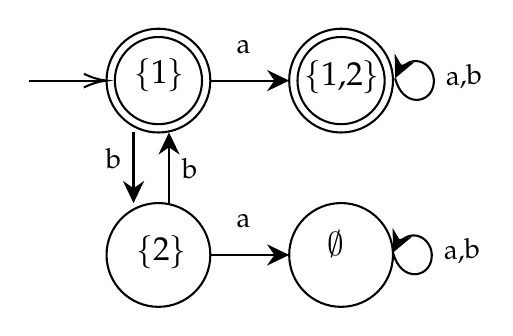
\begin{tikzpicture}[x=0.75pt,y=0.75pt,yscale=-1,xscale=1]
%uncomment if require: \path (0,165); %set diagram left start at 0, and has height of 165

%Shape: Circle [id:dp041480297844396885] 
\draw   (55,37) .. controls (55,23.19) and (66.19,12) .. (80,12) .. controls (93.81,12) and (105,23.19) .. (105,37) .. controls (105,50.81) and (93.81,62) .. (80,62) .. controls (66.19,62) and (55,50.81) .. (55,37) -- cycle ;
%Straight Lines [id:da13899408344347086] 
\draw    (17.5,37) -- (53,37) ;
\draw [shift={(55,37)}, rotate = 180] [color={rgb, 255:red, 0; green, 0; blue, 0 }  ][line width=0.75]    (10.93,-3.29) .. controls (6.95,-1.4) and (3.31,-0.3) .. (0,0) .. controls (3.31,0.3) and (6.95,1.4) .. (10.93,3.29)   ;
%Shape: Circle [id:dp8612999866988764] 
\draw   (143,37) .. controls (143,23.19) and (154.19,12) .. (168,12) .. controls (181.81,12) and (193,23.19) .. (193,37) .. controls (193,50.81) and (181.81,62) .. (168,62) .. controls (154.19,62) and (143,50.81) .. (143,37) -- cycle ;
%Straight Lines [id:da9417067835910866] 
\draw    (105,37) -- (140,37) ;
\draw [shift={(143,37)}, rotate = 180] [fill={rgb, 255:red, 0; green, 0; blue, 0 }  ][line width=0.08]  [draw opacity=0] (10.72,-5.15) -- (0,0) -- (10.72,5.15) -- (7.12,0) -- cycle    ;
%Shape: Circle [id:dp3667412328345818] 
\draw   (55,121) .. controls (55,107.19) and (66.19,96) .. (80,96) .. controls (93.81,96) and (105,107.19) .. (105,121) .. controls (105,134.81) and (93.81,146) .. (80,146) .. controls (66.19,146) and (55,134.81) .. (55,121) -- cycle ;
%Shape: Circle [id:dp7426517097906689] 
\draw   (143,121) .. controls (143,107.19) and (154.19,96) .. (168,96) .. controls (181.81,96) and (193,107.19) .. (193,121) .. controls (193,134.81) and (181.81,146) .. (168,146) .. controls (154.19,146) and (143,134.81) .. (143,121) -- cycle ;
%Straight Lines [id:da6063327159577332] 
\draw    (68,62) -- (68,93) ;
\draw [shift={(68,96)}, rotate = 270] [fill={rgb, 255:red, 0; green, 0; blue, 0 }  ][line width=0.08]  [draw opacity=0] (10.72,-5.15) -- (0,0) -- (10.72,5.15) -- (7.12,0) -- cycle    ;
%Straight Lines [id:da4625666754527742] 
\draw    (105,121) -- (140,121) ;
\draw [shift={(143,121)}, rotate = 180] [fill={rgb, 255:red, 0; green, 0; blue, 0 }  ][line width=0.08]  [draw opacity=0] (10.72,-5.15) -- (0,0) -- (10.72,5.15) -- (7.12,0) -- cycle    ;
%Straight Lines [id:da6471909245484817] 
\draw    (85.1,96) -- (85.1,65) ;
\draw [shift={(85.1,62)}, rotate = 450] [fill={rgb, 255:red, 0; green, 0; blue, 0 }  ][line width=0.08]  [draw opacity=0] (10.72,-5.15) -- (0,0) -- (10.72,5.15) -- (7.12,0) -- cycle    ;
%Curve Lines [id:da8907312304013146] 
\draw    (194.05,35.85) .. controls (197.65,50.35) and (211.65,48.35) .. (212.65,38.35) .. controls (213.58,29) and (202.28,22.27) .. (195.41,33.29) ;
\draw [shift={(194.05,35.85)}, rotate = 294.47] [fill={rgb, 255:red, 0; green, 0; blue, 0 }  ][line width=0.08]  [draw opacity=0] (10.72,-5.15) -- (0,0) -- (10.72,5.15) -- (7.12,0) -- cycle    ;
%Curve Lines [id:da00664507001788972] 
\draw    (193.05,119.85) .. controls (196.65,134.35) and (210.65,132.35) .. (211.65,122.35) .. controls (212.58,113) and (201.28,106.27) .. (194.41,117.29) ;
\draw [shift={(193.05,119.85)}, rotate = 294.47] [fill={rgb, 255:red, 0; green, 0; blue, 0 }  ][line width=0.08]  [draw opacity=0] (10.72,-5.15) -- (0,0) -- (10.72,5.15) -- (7.12,0) -- cycle    ;
%Shape: Circle [id:dp04204898944670221] 
\draw   (59,37) .. controls (59,25.4) and (68.4,16) .. (80,16) .. controls (91.6,16) and (101,25.4) .. (101,37) .. controls (101,48.6) and (91.6,58) .. (80,58) .. controls (68.4,58) and (59,48.6) .. (59,37) -- cycle ;
%Shape: Circle [id:dp5670937595756509] 
\draw   (147,37) .. controls (147,25.4) and (156.4,16) .. (168,16) .. controls (179.6,16) and (189,25.4) .. (189,37) .. controls (189,48.6) and (179.6,58) .. (168,58) .. controls (156.4,58) and (147,48.6) .. (147,37) -- cycle ;

% Text Node
\draw (67,25) node [anchor=north west][inner sep=0.75pt]  [font=\large] [align=left] {\{1\}};
% Text Node
\draw (149,26) node [anchor=north west][inner sep=0.75pt]  [font=\large] [align=left] {\{1,2\}};
% Text Node
\draw (68,110) node [anchor=north west][inner sep=0.75pt]  [font=\large] [align=left] {\{2\}};
% Text Node
\draw (160,108) node [anchor=north west][inner sep=0.75pt]  [font=\large] [align=left] {$\displaystyle \emptyset $};
% Text Node
\draw (53.11,67.99) node [anchor=north west][inner sep=0.75pt]  [rotate=-359.73] [align=left] {b};
% Text Node
\draw (116.11,15.99) node [anchor=north west][inner sep=0.75pt]  [rotate=-359.73] [align=left] {a};
% Text Node
\draw (116.11,99.99) node [anchor=north west][inner sep=0.75pt]  [rotate=-359.73] [align=left] {a};
% Text Node
\draw (89.94,73.04) node [anchor=north west][inner sep=0.75pt]  [rotate=-359.93] [align=left] {b};
% Text Node
\draw (216.87,27.96) node [anchor=north west][inner sep=0.75pt]  [rotate=-358.81] [align=left] {a,b};
% Text Node
\draw (215.87,111.96) node [anchor=north west][inner sep=0.75pt]  [rotate=-358.81] [align=left] {a,b};


\end{tikzpicture}

\item

\begin{tabular}{|c||c|c|}

$\delta'$ & $a$ & $b$ \\

\hline

$\{1,2\}$ & $\{1,2,3\}$ & $\varnothing$ \\

\hline

$\{1,2,3\}$ & $\{1,2,3\}$ & $\{1,2,3\}$ \\

\hline

$\varnothing$ & $\varnothing$ & $\varnothing$
\end{tabular}

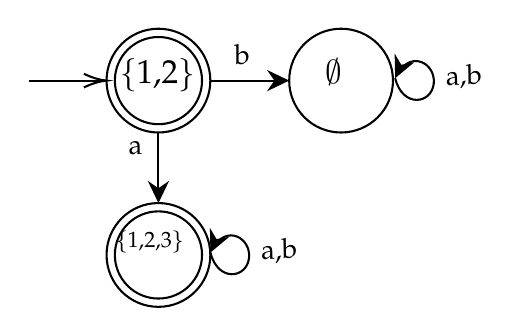
\begin{tikzpicture}[x=0.75pt,y=0.75pt,yscale=-1,xscale=1]
%uncomment if require: \path (0,163); %set diagram left start at 0, and has height of 163

%Shape: Circle [id:dp755149352320647] 
\draw   (58,37) .. controls (58,23.19) and (69.19,12) .. (83,12) .. controls (96.81,12) and (108,23.19) .. (108,37) .. controls (108,50.81) and (96.81,62) .. (83,62) .. controls (69.19,62) and (58,50.81) .. (58,37) -- cycle ;
%Straight Lines [id:da4413956565612509] 
\draw    (20.5,37) -- (56,37) ;
\draw [shift={(58,37)}, rotate = 180] [color={rgb, 255:red, 0; green, 0; blue, 0 }  ][line width=0.75]    (10.93,-3.29) .. controls (6.95,-1.4) and (3.31,-0.3) .. (0,0) .. controls (3.31,0.3) and (6.95,1.4) .. (10.93,3.29)   ;
%Shape: Circle [id:dp6756537097276512] 
\draw   (146,37) .. controls (146,23.19) and (157.19,12) .. (171,12) .. controls (184.81,12) and (196,23.19) .. (196,37) .. controls (196,50.81) and (184.81,62) .. (171,62) .. controls (157.19,62) and (146,50.81) .. (146,37) -- cycle ;
%Straight Lines [id:da7136395474545942] 
\draw    (108,37) -- (143,37) ;
\draw [shift={(146,37)}, rotate = 180] [fill={rgb, 255:red, 0; green, 0; blue, 0 }  ][line width=0.08]  [draw opacity=0] (10.72,-5.15) -- (0,0) -- (10.72,5.15) -- (7.12,0) -- cycle    ;
%Shape: Circle [id:dp4868575813671836] 
\draw   (58,121) .. controls (58,107.19) and (69.19,96) .. (83,96) .. controls (96.81,96) and (108,107.19) .. (108,121) .. controls (108,134.81) and (96.81,146) .. (83,146) .. controls (69.19,146) and (58,134.81) .. (58,121) -- cycle ;
%Straight Lines [id:da6893183418629139] 
\draw    (83,62) -- (83,76.6) -- (83,93) ;
\draw [shift={(83,96)}, rotate = 270] [fill={rgb, 255:red, 0; green, 0; blue, 0 }  ][line width=0.08]  [draw opacity=0] (10.72,-5.15) -- (0,0) -- (10.72,5.15) -- (7.12,0) -- cycle    ;
%Curve Lines [id:da4627577567750265] 
\draw    (197.05,35.85) .. controls (200.65,50.35) and (214.65,48.35) .. (215.65,38.35) .. controls (216.58,29) and (205.28,22.27) .. (198.41,33.29) ;
\draw [shift={(197.05,35.85)}, rotate = 294.47] [fill={rgb, 255:red, 0; green, 0; blue, 0 }  ][line width=0.08]  [draw opacity=0] (10.72,-5.15) -- (0,0) -- (10.72,5.15) -- (7.12,0) -- cycle    ;
%Curve Lines [id:da1057877531443927] 
\draw    (108.05,119.85) .. controls (111.65,134.35) and (125.65,132.35) .. (126.65,122.35) .. controls (127.58,113) and (116.28,106.27) .. (109.41,117.29) ;
\draw [shift={(108.05,119.85)}, rotate = 294.47] [fill={rgb, 255:red, 0; green, 0; blue, 0 }  ][line width=0.08]  [draw opacity=0] (10.72,-5.15) -- (0,0) -- (10.72,5.15) -- (7.12,0) -- cycle    ;
%Shape: Circle [id:dp44172249993130097] 
\draw   (62,121) .. controls (62,109.4) and (71.4,100) .. (83,100) .. controls (94.6,100) and (104,109.4) .. (104,121) .. controls (104,132.6) and (94.6,142) .. (83,142) .. controls (71.4,142) and (62,132.6) .. (62,121) -- cycle ;
%Shape: Circle [id:dp24374068945237215] 
\draw   (62,37) .. controls (62,25.4) and (71.4,16) .. (83,16) .. controls (94.6,16) and (104,25.4) .. (104,37) .. controls (104,48.6) and (94.6,58) .. (83,58) .. controls (71.4,58) and (62,48.6) .. (62,37) -- cycle ;

% Text Node
\draw (63,25) node [anchor=north west][inner sep=0.75pt]  [font=\large] [align=left] {\{1,2\}};
% Text Node
\draw (61,108) node [anchor=north west][inner sep=0.75pt]  [font=\large] [align=left] {{\footnotesize \{1,2,3\}}};
% Text Node
\draw (162,25) node [anchor=north west][inner sep=0.75pt]  [font=\large] [align=left] {$\displaystyle \emptyset $};
% Text Node
\draw (67.11,64.99) node [anchor=north west][inner sep=0.75pt]  [rotate=-359.73] [align=left] {a};
% Text Node
\draw (118.11,17.99) node [anchor=north west][inner sep=0.75pt]  [rotate=-359.73] [align=left] {b};
% Text Node
\draw (219.87,27.96) node [anchor=north west][inner sep=0.75pt]  [rotate=-358.81] [align=left] {a,b};
% Text Node
\draw (130.87,111.96) node [anchor=north west][inner sep=0.75pt]  [rotate=-358.81] [align=left] {a,b};


\end{tikzpicture}


\end{enumerate}

\end{document}
